% !TeX program = xelatex
% !Mode:: "TeX:UTF-8"
%%  本模板推荐以下方式编译: xelatex
%%     1. 文件默认的编码为 UTF-8 对于windows,请选用支持UTF-8编码的编辑器。
%%   2. 若是模板有什么问题,请及时与我们取得联系,Email:latexstudio@qq.com。
%%   3. 可以到  https://ask.latexstudio.net 提问
%%   4. 请安装 最新版本的 TeXLive 地址:
%%   http://mirrors.ctan.org/systems/texlive/Images/texlive.iso

\documentclass[12pt,a4paper]{nmmcm}
\usepackage{ctex}
\usepackage{graphicx}
\usepackage{booktabs,colortbl}
\usepackage{xcolor}
\usepackage{tikz}
\usepackage{indentfirst}
\usepackage{textcomp}
\usepackage{float}
\mcmsetup{CTeX = true,
        tcn = 2023051018408 , problem = A,
        sheet = true, titleinsheet = false, keywordsinsheet = true,
        titlepage = true, abstract = true}
\usepackage{xurl}
\setmainfont{Times New Roman}
\setmonofont[
    Path=fonts/,
    UprightFont = *-Regular,
    BoldFont = *-Bold,
    ItalicFont = *-Italic
]{UbuntuMono}
\usepackage{lipsum}


\usepackage{paralist}
\let\itemize\compactitem
\let\enditemize\endcompactitem
\let\enumerate\compactenum
\let\endenumerate\endcompactenum
\let\description\compactdesc
\let\enddescription\endcompactdesc

\setlength\abovedisplayskip{5pt}
\setlength\belowdisplayskip{-8pt}
\setlength{\parskip}{0.1em}

\newcommand\wordc[1]{\textbf{#1}}
\renewcommand{\appendixtocname}{附\quad录}
\renewcommand{\appendices}{\hspace{-2em}{\sanhao\HEI {\bf 附~~~录}}}
\colorlet{tableheadcolor}{gray!25} % Table header colour = 25% gray
\newcommand{\headcol}{\rowcolor{tableheadcolor}}

\title{列车能耗优化问题研究}
\date{}

\usepackage[font=small,labelfont={bf,sf},tableposition=top]{caption}


\begin{document}
\begin{abstract}


%abstract---------------
随着城市交通电气化进程的快速推进,城市轨道交通的能耗快速增长,城轨系统需求侧响应成为了一种有效的降低牵引能耗成本的手段。本文针对城轨系统的能耗问题,探讨了不同运行策略对能源消耗的影响,通过分析列车运行过程中的路段坡度、速度限速等因素,建立了列车消耗能量优化模型,并结合栅格化蚁群算法进行优化求解。

针对问题一,我们将列车运行阶段进行划分并分别建立距离,速度与时间的微分方程,通过4阶龙格库塔法求其数值解。考虑列车在最短时间上增加运行时间的运行速度轨迹,并画出分别增加10s、20s、50s、150s、300s的速度-距离曲线、牵引制动力-距离曲线、时间-距离曲线与能量消耗-距离曲线。

针对问题二,我们将路段进行划分并栅格化,利用栅格化蚁群算法对其进行求解,得到使运行过程能耗降低的可行的速度轨迹。在考虑路况信息情况下利用问题一模型求解得到列车最短运行时间的速度轨迹。根据问题一,画出列车以最短时间到达站台 B、在最短运行时间上分别增加 10s、20s、50s、150s、300s 到达站台 B的6组曲线。

针对问题三,我们将列车匀速运行分为两个阶段来降低列车在匀速阶段行驶距离,使得列车能够在原计划基础上延迟60s到达终点,并且对运行方案进行优化,得到优化后的运行速度轨迹并做出优化后列车运行过程的速度-距离曲线、牵引制动力-距离曲线、时间-距离曲线与能量消耗-距离曲线。







\begin{keywords}
{\song\xiaosihao
{列车能耗优化;龙格库塔法;栅格化蚁群算法}}
\end{keywords}
\end{abstract}
\maketitle
\renewcommand{\contentsname}{\centerline{\sanhao\bfseries\HEI 目\quad 录}}
%\thispagestyle{empty}
%{\song\xiaosihao
\tableofcontents
%}

\newpage
\setcounter{page}{1}
\pagestyle{fancy}
\section{问题重述}
\subsection{问题背景}
城轨系统的需求侧响应可以在保证乘客满意度的情况下降低牵引能耗成本,可进一步发掘城轨系统减碳节能的潜力。在列车运行过程中,列车与外界会产生各种摩擦,消耗列车牵引的能量。因此,考虑列车与轨道的摩擦、列车受到的空气阻力、列车势能的变化、列车运行过程中的位置限速等因素,在同一段旅途中,使用不同的驾驶策略会产生不同的能量和时间的消耗。因此,需要通过数学建模的方法,探究列车运行过程中能耗消耗规律,为城轨系统减碳节能提供支持。
\subsection{问题提出}
问题一考虑在列车在水平轨道上运行的情况下,假设列车所受的阻力满足 Davis 阻
力方程$ f = x_1 + x_2v + x_3v^2$,要求我们求解列车最短运行时间等情况下列车
运行过程的速度-距离曲线,牵引制动力-距离曲线,时间-距离曲线与能量消
耗-距离曲线共 6 组曲线。

问题二在问题一基础上,考虑动态过程,要求设计优化方案得到可行的速度轨迹使得列车能耗降低。参照问题一做出列车以最短运行时间等情况下的速度-距离曲线、牵
引制动力-距离曲线、时间-距离曲线和能量消耗-距离曲线。

问题三中列车由于前方突发事故的原因,需要在原定基础上延迟60s到达终点,需要设计优化方案在保持列车节能运行下较快地得到调整后的优化速度轨迹,并做出调整后列车运行过程的速度-距离曲线、牵引制动力-距离曲线、时间-距离曲线和能量消耗-距离曲线。
\section{问题分析}
\subsection{对问题一的分析}
题目给出了列车部分参数,并且假设列车所受的阻力满足Davis阻力方程,我们首先求解列车最短运行时间。分析可知列车在最大速度上行驶时间需要尽量长,也即列车加速阶段和减速阶段运行时间需要尽可能短,这样我们就得出了列车在最短运行时间情况下的三个运行阶段:加速阶段,匀速阶段和减速阶段。我们运用牛顿第二定律对列车进行受力分析,得出列车在各个阶段的速度-时间函数式,容易看出的是列车在加速阶段和减速阶段为非线性微分方程。我们对于非刚性微分方程问题,无法求出其解析解,可以采用微分方程的数值解法,例如龙格库塔法。再分别求解计算出其对应的距离,牵引制动力和耗费的能量并画出最短运行时间的一组曲线。

在最短时间上增加时间$T'$,我们考虑列车存在惰行阶段,即列车在水平方向上只受到阻力的作用。这时候我们有惰性阶段的起始时间和终止时间两个未知量,有运行距离不变和增加的运行时间两个方程,故理论上可以求出未知量的数值解。再求解计算出其变化后对应的距离,牵引制动力和耗费的能量并画出增加时间$T'$后的五组曲线。
\subsection{对问题二的分析}
考虑路况信息,在有限速条件和各路段坡度不同的情况下,要求设计优化方案使得运行过程的能耗降低。由于各路段坡度不同,即使在其他参数都保持一致的情况下列车的能耗也不尽相同,例如在上坡阶段的牵引能耗大于在下坡阶段的牵引能耗。对于复杂的路况信息,我们无法建立微分方程模型对其进行数值求解再去计算其能耗,考虑利用蚁群算法等智能算法对其进行仿真求解。我们首先将路段根据坡度和限速分为不同的路段,将各路段能耗总和最低作为目标函数,再对各路段进行栅格化,利用蚁群算法求解目标函数最小值,这样我们就可以得到使列车运行能耗降低的可行的速度轨迹。

参照问题一考虑列车的最短运行时间,在路段限速由$v_{max}$降低至$v'_{max}$前进入制动阶段使列车恰好在此路段到达最高限速,再以此速度进入匀速行驶阶段最后进行制动阶段。再根据问题一的求解方法得到最短运行时间的一组曲线。

在最短时间上增加时间$T'$,我们考虑列车在最后的减速阶段前进入惰行阶段,分别求出其数值解。再求解计算出其变化后对应的距离,牵引制动力和耗费的能量并画出增加时间$T'$后的五组曲线。
\subsection{对问题三的分析}
问题三要求我们再原计划基础上,由于突发事故需要延迟60s到达终点,设计优化方案使得列车保持节能运行情况下得到调整后的优化速度轨迹,并做出列车运行过程的曲线组。我们首先应该根据列车原计划运行时间确定列车可能的速度轨迹,在这里我们考虑改变列车匀速行驶阶段的速度来确定列车的运行速度轨迹使得列车恰好在原计划时间到达站点B。我们在问题一模型的基础上,考虑到要尽可能保持列车节能运行,又由问题二模型可知列车在惰行阶段的能耗最低,又因为减速阶段所运行的距离太短,我们需要考虑提前进入惰行阶段再进入匀速阶段最后再经过减速阶段或是惰行阶段到达站点B。又考虑到需要快速得到调整后的优化速度轨迹,注意到如果将减速阶段分到不同的时间点,它们的积分值即减速阶段运行的距离不会发生改变,我们可以通过数值积分得到这个距离。这样我们就可以让列车提前进入减速阶段,这样我们只需要确定原计划匀速行驶阶段还需行驶的距离再除以原计划匀速行驶阶段剩余时间和延迟的时间就可以得到列车调整后的优化速度轨迹。我们再利用问题一模型得到列车运行过程各参数作出列车运行过程的曲线组。
\section{模型假设}
\begin{enumerate}
  \item 列车工况间可以自由转化,即允许列车在匀速阶段下进入减速阶段
  \item 由于没有给定列车长度,我们将列车当作单质点进行计算
\end{enumerate}

\section{符号说明}
%tab1
\begin{table}[h!]
  \centering
  \small
  \begin{tabular}{p{60pt}<{\centering}|p{60pt}<{\centering}p{180pt}<{\raggedright}}
   \hline
   \headcol 序号 & 符号 & 符号说明 \\
   \hline
    1 & $\mathbf{D}$ & 微分算子 \\
    2 & $X_n$ & 路段n \\
    3 & $\theta$ & 坡度($\textperthousand$) \\
    4 & $E_X$ & 列车能耗 \\
    5 & $v_{{X_n}_{max}}$ & 列车在路段$X_n$所允许的最大速率 \\
    \hline
  \end{tabular}
  %\caption{符号与说明}
  \label{symbol}
\end{table}
\clearpage
\section{问题一模型的建立与求解}

% 数据的预处理:
% 1. $\cdots\cdots$数据全部缺失,不予考虑。
% 2. 对数据测试的特点,如周期等进行分析。
% 3. $\cdots\cdots$数据残缺,根据数据挖掘等理论根据$\cdots\cdots$变化趋势进行补充。
% 4. 对数据特点(后面将会用到的特征)进行提取。
%    用$\cdots\cdots$软件聚类分析和各个不同问题的需要,采得$\cdots\cdots$组采样,每组5-8个采样值。将采样所对应的特征值进行列表或图示。
% 根据数据特点,对总体和个体的特点进行比较,以表格或图示方式显示。


% \subsection{问题一的分析和求解}

% \subsubsection{***模型的建立}

% 模型建立的内容要点如下:

% 模型的主要类别:

% 几种常见的建模目的:

% 建模过程常见的几个要点:

% 模型的基本要求:

% 模型选择要点:

% 加分项(能在规定时间内做完后还有足够时间的再考虑加分项):

% 1、鼓励创新。在能解决问题的基础上,对经典模型进行改进,欣赏独树一帜、有创新性的模型,但要合理。

% 2、对于同一问题使用两个或以上合理模型进行求解。避免出现单纯罗列模型,又不做对比和评价的现象。

% \begin{figure}[h!t]
% \centerline{
% \begin{tikzpicture}[scale=0.6]
%   \foreach \y [count=\n] in {
%       {74,25,39,20,3,3,3,3,3},
%       {25,53,31,17,7,7,2,3,2},
%       {39,31,37,24,3,3,3,3,3},
%       {20,17,24,37,2,2,6,5,5},
%       {3,7,3,2,12,1,0,0,0},
%       {3,7,3,2,1,36,0,0,0},
%       {3,2,3,6,0,0,45,1,1},
%       {3,3,3,5,0,0,1,23,1},
%       {3,2,3,5,0,0,1,1,78},
%     } {
%       \foreach \x [count=\m] in \y {
%         \node[fill=yellow!\x!blue, minimum size=6mm, text=white] at (\m,-\n) {\x};
%       }
%     }
% \end{tikzpicture}\quad
% \begin{tikzpicture}[scale=0.6]
%   \foreach \y [count=\n] in {
%       {74,25,39,20,3,3,3,3,3},
%       {25,53,31,17,7,7,2,3,2},
%       {39,31,37,24,3,3,3,3,3},
%       {20,17,24,37,2,2,6,5,5},
%       {3,7,3,2,12,1,0,0,0},
%       {3,7,3,2,1,36,0,0,0},
%       {3,2,3,6,0,0,45,1,1},
%       {3,3,3,5,0,0,1,23,1},
%       {3,2,3,5,0,0,1,1,78},
%     } {
%       \foreach \x [count=\m] in \y {
%         \node[fill=yellow!\x!purple, minimum size=6mm, text=white] at (\m,-\n) {\x};
%       }
%     }
% \end{tikzpicture}
% }
% \caption{图~2的标题名称}
% \end{figure}



% 参考话术:我们需要解决的问题是$\cdots\cdots$,题目要求是$\cdots\cdots$,剔除$\cdots\cdots$数据后选用何种类型的模型优点进行分析。具体步骤123$\cdots$
我们设列车行驶距离为$s(s\le 5144.7m)$,运行速度的上限为$v_{max}$,列车质量为$m$,列车最大牵引力为$F_{Q}$,机械制动部分最大制动力为$F_Z$。我们先考虑让列车运行时间最短情况下。分析可知,需让列车在最大速率$v_{max}$情况下运行时间最长,即让列车在加速和减速阶段运行时间最短,我们画出示意图如下:
\begin{figure}[H]
\centering
\tikzset{every picture/.style={line width=0.75pt}} %set default line width to 0.75pt        

\begin{tikzpicture}[x=0.75pt,y=0.75pt,yscale=-1,xscale=1]
%uncomment if require: \path (0,235); %set diagram left start at 0, and has height of 235

%Straight Lines [id:da37990160478338986] 
\draw    (99.79,201.3) -- (99.79,52.3) ;
\draw [shift={(99.79,50.3)}, rotate = 90] [color={rgb, 255:red, 0; green, 0; blue, 0 }  ][line width=0.75]    (10.93,-3.29) .. controls (6.95,-1.4) and (3.31,-0.3) .. (0,0) .. controls (3.31,0.3) and (6.95,1.4) .. (10.93,3.29)   ;
%Straight Lines [id:da40399304010443426] 
\draw    (99.79,201.3) -- (348.05,200.77) ;
\draw [shift={(350.05,200.76)}, rotate = 179.88] [color={rgb, 255:red, 0; green, 0; blue, 0 }  ][line width=0.75]    (10.93,-3.29) .. controls (6.95,-1.4) and (3.31,-0.3) .. (0,0) .. controls (3.31,0.3) and (6.95,1.4) .. (10.93,3.29)   ;
%Curve Lines [id:da15310766962725486] 
\draw    (99.79,201.3) .. controls (107.96,142.63) and (111.91,125.26) .. (175.29,123.96) ;
%Straight Lines [id:da8929712953501876] 
\draw    (175.29,123.96) -- (249.96,123.96) ;
%Curve Lines [id:da4544129298714623] 
\draw    (249.96,123.96) .. controls (261.29,163.96) and (263.29,199.29) .. (309.96,200.63) ;
%Straight Lines [id:da3508839243427788] 
\draw  [dash pattern={on 0.84pt off 2.51pt}]  (170.71,123.96) -- (170.04,201.29) ;
%Straight Lines [id:da16767314879407658] 
\draw  [dash pattern={on 0.84pt off 2.51pt}]  (249.96,123.96) -- (250.04,200.63) ;
%Straight Lines [id:da6854846814598163] 
\draw  [dash pattern={on 0.84pt off 2.51pt}]  (103.37,123.96) -- (170.71,123.96) ;

% Text Node
\draw (86,46) node [anchor=north west][inner sep=0.75pt]   [align=left] {$\displaystyle v$};
% Text Node
\draw (338,205.33) node [anchor=north west][inner sep=0.75pt]   [align=left] {$\displaystyle t$};
% Text Node
\draw (162.67,204) node [anchor=north west][inner sep=0.75pt]   [align=left] {$\displaystyle t_{0}$};
% Text Node
\draw (243.33,203.33) node [anchor=north west][inner sep=0.75pt]   [align=left] {$\displaystyle t_{1}$};
% Text Node
\draw (62,112.33) node [anchor=north west][inner sep=0.75pt]   [align=left] {$\displaystyle v_{max}$};
% Text Node
\draw (84.67,202.33) node [anchor=north west][inner sep=0.75pt]   [align=left] {$\displaystyle O$};
\draw (300.67,202.33) node [anchor=north west][inner sep=0.75pt]   [align=left] {$\displaystyle T$};

\end{tikzpicture}
\caption{最短时间的$v$-$t$曲线}
\end{figure}

其中,$t_0$表示列车从静止开始加速到最大加速度的时刻,$t_1$为列车开始减速的时刻,$T$为列车到达站点B的时刻。我们将列车运行分为三个阶段:加速阶段,匀速行驶阶段和减速阶段。分别讨论如下:
\subsection{加速阶段}
\begin{figure}[H]
\centering
\resizebox{\textwidth}{!}{
\tikzset{every picture/.style={line width=0.75pt}} %set default line width to 0.75pt        

\begin{tikzpicture}[x=0.75pt,y=0.75pt,yscale=-1,xscale=1]
%uncomment if require: \path (0,488); %set diagram left start at 0, and has height of 488

%Image [id:dp8849655169521458] 
\draw (322.64,179.89) node  {\includegraphics[width=412.96pt,height=170.34pt]{图片1.png}};
%Straight Lines [id:da5502193869444818] 
\draw [line width=1.5]    (323.62,200.38) -- (53.96,199.72) ;
\draw [shift={(50.96,199.71)}, rotate = 0.14] [color={rgb, 255:red, 0; green, 0; blue, 0 }  ][line width=1.5]    (9.95,-2.99) .. controls (6.32,-1.27) and (3.01,-0.27) .. (0,0) .. controls (3.01,0.27) and (6.32,1.27) .. (9.95,2.99)   ;
\draw [shift={(323.62,200.38)}, rotate = 180.14] [color={rgb, 255:red, 0; green, 0; blue, 0 }  ][fill={rgb, 255:red, 0; green, 0; blue, 0 }  ][line width=1.5]      (0, 0) circle [x radius= 3.05, y radius= 3.05]   ;
%Straight Lines [id:da6131591626000272] 
\draw [line width=1.5]    (323.62,200.38) -- (696.62,201.04) ;
\draw [shift={(699.62,201.04)}, rotate = 180.1] [color={rgb, 255:red, 0; green, 0; blue, 0 }  ][line width=1.5]    (14.21,-4.28) .. controls (9.04,-1.82) and (4.3,-0.39) .. (0,0) .. controls (4.3,0.39) and (9.04,1.82) .. (14.21,4.28)   ;
%Straight Lines [id:da18206739586388987] 
\draw [line width=1.5]    (258.95,155.12) -- (433.95,155.12) ;
\draw [shift={(436.95,155.12)}, rotate = 180] [color={rgb, 255:red, 0; green, 0; blue, 0 }  ][line width=1.5]    (14.21,-4.28) .. controls (9.04,-1.82) and (4.3,-0.39) .. (0,0) .. controls (4.3,0.39) and (9.04,1.82) .. (14.21,4.28)   ;

% Text Node
\draw (334.67,129) node [anchor=north west][inner sep=0.75pt]  [font=\large] [align=left] {$\displaystyle a_{1}$};
% Text Node
\draw (52.96,202.71) node [anchor=north west][inner sep=0.75pt]  [font=\large] [align=left] {$\displaystyle f$};
% Text Node
\draw (672.67,202.67) node [anchor=north west][inner sep=0.75pt]  [font=\large] [align=left] {$\displaystyle F_{Q}$};
% Text Node
\draw (512.95,165.58) node [anchor=north west][inner sep=0.75pt]  [font=\large] [align=left] {$\displaystyle m$};


\end{tikzpicture}}
\caption{加速阶段列车受力分析}
\end{figure}
列车以最大牵引力从静止开始启动,此时$t\in [0,t_0)$,由牛顿第二定律,我们有:
\begin{eqnarray}
F_Q-f=ma_1
\end{eqnarray}
\begin{eqnarray}
f=x_1+x_2v+x_3v^2
\end{eqnarray}
\begin{eqnarray}
v(t)=v(t-\Delta t)+a_1\Delta t\label{1}
\end{eqnarray}

我们再对公式\ref{1}两端积分有:
\begin{eqnarray}
s(t)=s(t-\Delta t)+v(t)\Delta t
\end{eqnarray}
\subsection{匀速阶段}
\begin{figure}[H]
\centering
\resizebox{\textwidth}{!}{


\tikzset{every picture/.style={line width=0.75pt}} %set default line width to 0.75pt        

\begin{tikzpicture}[x=0.75pt,y=0.75pt,yscale=-1,xscale=1]
%uncomment if require: \path (0,488); %set diagram left start at 0, and has height of 488

%Image [id:dp8849655169521458] 
\draw (321.31,179.89) node  {\includegraphics[width=412.96pt,height=170.34pt]{图片1.png}};
%Straight Lines [id:da5502193869444818] 
\draw [line width=1.5]    (323.62,200.38) -- (49.96,199.72) ;
\draw [shift={(46.96,199.71)}, rotate = 0.14] [color={rgb, 255:red, 0; green, 0; blue, 0 }  ][line width=1.5]    (9.95,-2.99) .. controls (6.32,-1.27) and (3.01,-0.27) .. (0,0) .. controls (3.01,0.27) and (6.32,1.27) .. (9.95,2.99)   ;
\draw [shift={(323.62,200.38)}, rotate = 180.14] [color={rgb, 255:red, 0; green, 0; blue, 0 }  ][fill={rgb, 255:red, 0; green, 0; blue, 0 }  ][line width=1.5]      (0, 0) circle [x radius= 3.05, y radius= 3.05]   ;
%Straight Lines [id:da6131591626000272] 
\draw [line width=1.5]    (323.62,200.38) -- (595.29,200.38) ;
\draw [shift={(598.29,200.38)}, rotate = 180] [color={rgb, 255:red, 0; green, 0; blue, 0 }  ][line width=1.5]    (14.21,-4.28) .. controls (9.04,-1.82) and (4.3,-0.39) .. (0,0) .. controls (4.3,0.39) and (9.04,1.82) .. (14.21,4.28)   ;

% Text Node
\draw (48.96,202.71) node [anchor=north west][inner sep=0.75pt]  [font=\large] [align=left] {$\displaystyle f$};
% Text Node
\draw (572.67,202.67) node [anchor=north west][inner sep=0.75pt]  [font=\large] [align=left] {$\displaystyle F_{Q}$};
% Text Node
\draw (512.95,165.58) node [anchor=north west][inner sep=0.75pt]  [font=\large] [align=left] {$\displaystyle m$};
% Text Node
\draw (295.33,153.33) node [anchor=north west][inner sep=0.75pt]  [font=\large] [align=left] {$\displaystyle a=0$};


\end{tikzpicture}
}\caption{匀速阶段列车受力分析}
\end{figure}
此阶段列车达到最大速率,此时列车加速度为0,$t\in [t_0,t_1]$由受力平衡有:
\begin{eqnarray}
v(t)=v_{max}
\end{eqnarray}
\begin{eqnarray}
s(t)=s(t_0)+(t-t_0)v_{max}
\end{eqnarray}
\subsection{减速阶段}
\begin{figure}[H]
\centering
\resizebox{\textwidth}{!}{




\tikzset{every picture/.style={line width=0.75pt}} %set default line width to 0.75pt        

\begin{tikzpicture}[x=0.75pt,y=0.75pt,yscale=-1,xscale=1]
%uncomment if require: \path (0,488); %set diagram left start at 0, and has height of 488

%Image [id:dp8849655169521458] 
\draw (323.31,179.89) node  {\includegraphics[width=412.96pt,height=170.34pt]{图片1.png}};
%Straight Lines [id:da5502193869444818] 
\draw [line width=1.5]    (323.62,200.38) -- (49.96,199.72) ;
\draw [shift={(46.96,199.71)}, rotate = 0.14] [color={rgb, 255:red, 0; green, 0; blue, 0 }  ][line width=1.5]    (9.95,-2.99) .. controls (6.32,-1.27) and (3.01,-0.27) .. (0,0) .. controls (3.01,0.27) and (6.32,1.27) .. (9.95,2.99)   ;
\draw [shift={(323.62,200.38)}, rotate = 180.14] [color={rgb, 255:red, 0; green, 0; blue, 0 }  ][fill={rgb, 255:red, 0; green, 0; blue, 0 }  ][line width=1.5]      (0, 0) circle [x radius= 3.05, y radius= 3.05]   ;
%Straight Lines [id:da6131591626000272] 
\draw [line width=1.5]    (323.62,200.38) -- (92.62,199.72) ;
\draw [shift={(89.62,199.71)}, rotate = 0.16] [color={rgb, 255:red, 0; green, 0; blue, 0 }  ][line width=1.5]    (14.21,-4.28) .. controls (9.04,-1.82) and (4.3,-0.39) .. (0,0) .. controls (4.3,0.39) and (9.04,1.82) .. (14.21,4.28)   ;
%Straight Lines [id:da6590127524837075] 
\draw [line width=1.5]    (382.96,151.71) -- (204.62,151.06) ;
\draw [shift={(201.62,151.04)}, rotate = 0.21] [color={rgb, 255:red, 0; green, 0; blue, 0 }  ][line width=1.5]    (17.05,-5.13) .. controls (10.84,-2.18) and (5.16,-0.47) .. (0,0) .. controls (5.16,0.47) and (10.84,2.18) .. (17.05,5.13)   ;

% Text Node
\draw (91.62,202.71) node [anchor=north west][inner sep=0.75pt]  [font=\large] [align=left] {$\displaystyle f$};
% Text Node
\draw (48.96,202.71) node [anchor=north west][inner sep=0.75pt]  [font=\large] [align=left] {$\displaystyle F_{Z}$};
% Text Node
\draw (512.95,165.58) node [anchor=north west][inner sep=0.75pt]  [font=\large] [align=left] {$\displaystyle m$};
% Text Node
\draw (245.33,125.33) node [anchor=north west][inner sep=0.75pt]  [font=\large] [align=left] {$\displaystyle a_{2}$};


\end{tikzpicture}

}\caption{减速阶段列车受力分析}
\end{figure}
在此阶段,列车以最大制动力进入减速阶段,此时$t\in(t_1,T]$,由牛顿第二定律有:
\begin{eqnarray}
f+F_Z=ma_2
\end{eqnarray}
\begin{eqnarray}
v(t)=v(t-\Delta t)-a_2\Delta t
\end{eqnarray}
\begin{eqnarray}
s(t)=s(t_1)+s(t-\Delta t)-v(t)\Delta t
\end{eqnarray}

在上面的分析中,我们就得到了速率关于时间和距离关于时间的两个函数表达式:
\begin{eqnarray}
v(t)=\left\{\begin{matrix}
 v(t-\Delta t)+a_1\Delta t &t\in[0,t_0) \\
 v_{max} &t\in [t_0,t_1] \\
  v(t-\Delta t)-a_2\Delta t&t\in (t_1,T]
\end{matrix}\right.
\end{eqnarray}
\begin{eqnarray}
s(t)=\left\{\begin{matrix}
 s(t-\Delta t)+v(t)\Delta t &t\in[0,t_0) \\
 s(t_0)+(t-t_0)v_{max} &t\in [t_0,t_1] \\
  s(t_1)+s(t-\Delta t)-v(t)\Delta t&t\in (t_1,T]
\end{matrix}\right.
\end{eqnarray}

可以看出上述函数为非线性的微分方程,我们在$t\in[0,t_0)\cup(t_1,T]$时刻对以上函数进行积分有:
\begin{eqnarray}
v(t)=\left\{\begin{matrix}
 \int_0^t\frac{F_Q-x_1-x_2v(t)-x_3v^2(t)}{m}\mathrm{d}t &t\in[0,t_0) \\
 v_{max} &t\in [t_0,t_1] \\
  v_{max}-\int_{t_1}^{t}\frac{F_Z+x_1+x_2v(t)+x_3v^2(t)}{m}\mathrm{d}t &t\in (t_1,T]
\end{matrix}\right.
\end{eqnarray}

\begin{eqnarray}
s(t)=\left\{\begin{matrix}
 \int_0^tv(t) \mathrm{d}t &t\in[0,t_0) \\
 s(t_0)+(t-t_0)v_{max} &t\in [t_0,t_1] \\
  s(t_1)+\int_{t_1}^tv(t)\mathrm{d}t&t\in (t_1,T]
\end{matrix}\right.
\end{eqnarray}

我们设列车总消耗的能量为$E_X$,由于阻力所消耗的能量为$E_f$,列车制动所消耗的能量为$E_Z$,易得:
\begin{eqnarray}
E_f(t)=f\cdot s(t)
\end{eqnarray}
\begin{eqnarray}
E_Z(t)=F_Z(t)\cdot \max\{s(t)-s(t_1),0\}
\end{eqnarray}

则我们由动能定理有:
\begin{eqnarray}
\frac{1}{2}mv^2-0=E_X-E_f-E_Z
\end{eqnarray}

整理得:
\begin{eqnarray}
E_X(t)=\frac{1}{2}mv^2(t)+E_f(t)+E_Z(t)
\end{eqnarray}

可以看出在列车所受阻力满足Davis阻力方程情况下,我们的微分方程$\mathbf{D}{v(t)}=\phi (v(t))$中$v(t)$最高次数为2次,说明该微分方程并非线性的,故我们无法求得解析解。基于此,我们可以利用龙格库塔法求解该非刚性常微分方程组(ODEs)的解析解。
\subsection{龙格库塔法介绍}
龙格-库塔法是常用的一种求解常微分方程初值问题的数值方法。它利用迭代的方式逼近精确解,并具有一定的精度和稳定性。

对于一阶常微分方程$y'=f(x,y)$,初始条件为$y(x_0)=y_0$,龙格-库塔法的基本思路是在$x_0$处计算初始值$y_0$,然后在$x_0$处计算斜率$k_1=f(x_0,y_0)$,接着通过四个不同点的加权平均来计算下一个近似解$y_1$:
\begin{eqnarray}
\left\{\begin{matrix}
k_1=f(x_0,y_0) \\
k_2=f(x_0+\frac{h}{2},y_0+\frac{k_1h}{2}) \\
k_3=f(x_0+\frac{h}{2},y_0+\frac{k_2h}{2}) \\
k_4=f(x_0+h,y_0+k_3h) \\
y_1=y_0+\frac{h}{6}(k_1+2k_2+2k_3+k_4)
\end{matrix}\right.
\end{eqnarray}
其中,$h$为步长,可以根据需要调整。

使用龙格-库塔法,可以通过多次迭代来得到一个足够接近精确解的数值解,其精度通常比欧拉法更高。

这里我们将利用MATLAB自带的ode45函数进行求解并这组曲线展示在图\ref{zd}中:
\begin{figure}[H]
\centering
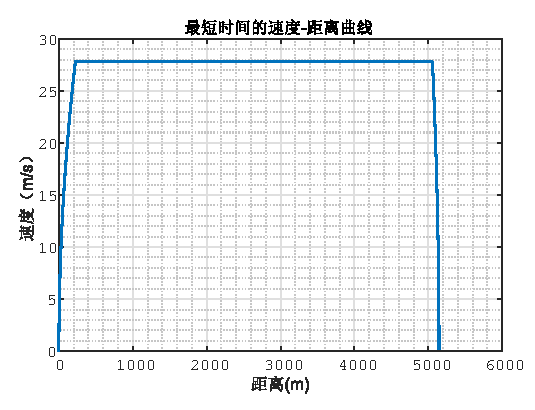
\includegraphics[width=.49\textwidth]{figures/a.eps}
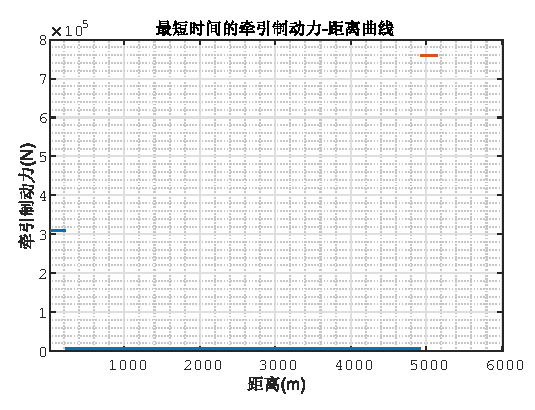
\includegraphics[width=.49\textwidth]{figures/b.eps}
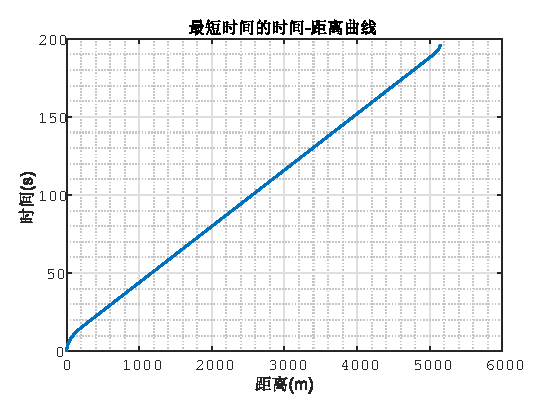
\includegraphics[width=.49\textwidth]{figures/c.eps}
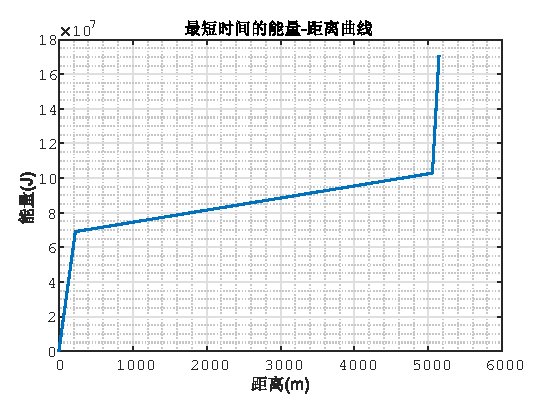
\includegraphics[width=.49\textwidth]{figures/d.eps}
\caption{\song\wuhao 最短时间的曲线组}\label{zd}
\end{figure}
\subsection{惰行阶段}
\begin{figure}[H]
\centering
\resizebox{\textwidth}{!}{
\tikzset{every picture/.style={line width=0.75pt}} %set default line width to 0.75pt        

\begin{tikzpicture}[x=0.75pt,y=0.75pt,yscale=-1,xscale=1]
%uncomment if require: \path (0,488); %set diagram left start at 0, and has height of 488

%Image [id:dp8849655169521458] 
\draw (323.31,179.89) node  {\includegraphics[width=412.96pt,height=170.34pt]{图片1.png}};
%Straight Lines [id:da5502193869444818] 
\draw [line width=1.5]    (323.62,200.38) -- (49.96,199.72) ;
\draw [shift={(46.96,199.71)}, rotate = 0.14] [color={rgb, 255:red, 0; green, 0; blue, 0 }  ][line width=1.5]    (9.95,-2.99) .. controls (6.32,-1.27) and (3.01,-0.27) .. (0,0) .. controls (3.01,0.27) and (6.32,1.27) .. (9.95,2.99)   ;
\draw [shift={(323.62,200.38)}, rotate = 180.14] [color={rgb, 255:red, 0; green, 0; blue, 0 }  ][fill={rgb, 255:red, 0; green, 0; blue, 0 }  ][line width=1.5]      (0, 0) circle [x radius= 3.05, y radius= 3.05]   ;
%Straight Lines [id:da6590127524837075] 
\draw [line width=1.5]    (382.96,151.71) -- (204.62,151.06) ;
\draw [shift={(201.62,151.04)}, rotate = 0.21] [color={rgb, 255:red, 0; green, 0; blue, 0 }  ][line width=1.5]    (17.05,-5.13) .. controls (10.84,-2.18) and (5.16,-0.47) .. (0,0) .. controls (5.16,0.47) and (10.84,2.18) .. (17.05,5.13)   ;

% Text Node
\draw (48.96,202.71) node [anchor=north west][inner sep=0.75pt]  [font=\large] [align=left] {$\displaystyle f$};
% Text Node
\draw (512.95,165.58) node [anchor=north west][inner sep=0.75pt]  [font=\large] [align=left] {$\displaystyle m$};
% Text Node
\draw (245.33,125.33) node [anchor=north west][inner sep=0.75pt]  [font=\large] [align=left] {$\displaystyle a_{3}$};


\end{tikzpicture}


}\caption{惰行阶段列车受力分析}
\end{figure}
在上述求解过程中,为了让列车运行时间最短,我们没有考虑列车进入惰性阶段,即列车牵引力和制动力全部降为0,只有运行阻力做功,记$F_D$为惰性阶段列车所受外力,我们有:
\begin{eqnarray}
F_D=-f
\end{eqnarray}
\begin{eqnarray}
F_D=ma_3
\end{eqnarray}

我们在最短时间上增加$T'$,我们就考虑在匀速阶段和减速阶段中间加入惰行阶段,列车运行时间增加变化的$v$-$t$曲线如下图所示:
\begin{figure}[H]
\centering
\resizebox{\textwidth}{!}{
\tikzset{every picture/.style={line width=0.75pt}} %set default line width to 0.75pt        

\begin{tikzpicture}[x=0.75pt,y=0.75pt,yscale=-1,xscale=1]
%uncomment if require: \path (0,586); %set diagram left start at 0, and has height of 586

%Straight Lines [id:da8476045734445774] 
\draw    (100.03,239.96) -- (100.03,82.63) ;
\draw [shift={(100.03,80.63)}, rotate = 90] [color={rgb, 255:red, 0; green, 0; blue, 0 }  ][line width=0.75]    (10.93,-3.29) .. controls (6.95,-1.4) and (3.31,-0.3) .. (0,0) .. controls (3.31,0.3) and (6.95,1.4) .. (10.93,3.29)   ;
%Straight Lines [id:da728488507189408] 
\draw    (100.03,239.96) -- (278.03,239.96) ;
\draw [shift={(280.03,239.96)}, rotate = 180] [color={rgb, 255:red, 0; green, 0; blue, 0 }  ][line width=0.75]    (10.93,-3.29) .. controls (6.95,-1.4) and (3.31,-0.3) .. (0,0) .. controls (3.31,0.3) and (6.95,1.4) .. (10.93,3.29)   ;
%Curve Lines [id:da4903463231770826] 
\draw    (100.03,239.96) .. controls (100.03,182.63) and (107.37,157.29) .. (140.7,150.63) ;
%Straight Lines [id:da760646461032279] 
\draw    (140.7,150.63) -- (210.03,150.63) ;
%Curve Lines [id:da6353141367423694] 
\draw    (210.03,150.63) .. controls (214.7,184.63) and (225.29,233.22) .. (254.62,239.88) ;
%Straight Lines [id:da7799521976525747] 
\draw  [dash pattern={on 0.84pt off 2.51pt}]  (99.96,150.55) -- (140.7,150.63) ;
%Straight Lines [id:da3342268810432476] 
\draw  [dash pattern={on 0.84pt off 2.51pt}]  (140.7,150.63) -- (139.96,239.22) ;
%Straight Lines [id:da5580021355048268] 
\draw  [dash pattern={on 0.84pt off 2.51pt}]  (210.03,150.63) -- (209.29,239.22) ;
%Straight Lines [id:da5451067637372045] 
\draw    (390.7,240.63) -- (390.7,83.29) ;
\draw [shift={(390.7,81.29)}, rotate = 90] [color={rgb, 255:red, 0; green, 0; blue, 0 }  ][line width=0.75]    (10.93,-3.29) .. controls (6.95,-1.4) and (3.31,-0.3) .. (0,0) .. controls (3.31,0.3) and (6.95,1.4) .. (10.93,3.29)   ;
%Straight Lines [id:da38958300445579575] 
\draw    (390.7,240.63) -- (657.96,240.55) ;
\draw [shift={(659.96,240.55)}, rotate = 179.98] [color={rgb, 255:red, 0; green, 0; blue, 0 }  ][line width=0.75]    (10.93,-3.29) .. controls (6.95,-1.4) and (3.31,-0.3) .. (0,0) .. controls (3.31,0.3) and (6.95,1.4) .. (10.93,3.29)   ;
%Curve Lines [id:da5528666254821606] 
\draw    (390.7,240.63) .. controls (390.7,183.29) and (398.03,157.96) .. (431.37,151.29) ;
%Straight Lines [id:da3458593742567946] 
\draw  [dash pattern={on 4.5pt off 4.5pt}]  (466.03,151.29) -- (500.7,151.29) ;
%Curve Lines [id:da43237051166426177] 
\draw  [dash pattern={on 4.5pt off 4.5pt}]  (500.7,151.29) .. controls (505.37,185.29) and (515.96,233.88) .. (545.29,240.55) ;
%Straight Lines [id:da9426033233385211] 
\draw  [dash pattern={on 0.84pt off 2.51pt}]  (390.62,151.22) -- (431.37,151.29) ;
%Straight Lines [id:da9570390483739564] 
\draw  [dash pattern={on 0.84pt off 2.51pt}]  (431.37,151.29) -- (430.62,239.88) ;
%Straight Lines [id:da07294608228115895] 
\draw  [dash pattern={on 0.84pt off 2.51pt}]  (500.7,151.29) -- (499.96,239.88) ;
%Striped Right Arrow [id:dp7138793138394022] 
\draw   (290,153) -- (322,153) -- (322,143) -- (350,163) -- (322,183) -- (322,173) -- (290,173) -- cycle ;\draw   (280,153) -- (282,153) -- (282,173) -- (280,173) -- cycle ;\draw   (284,153) -- (288,153) -- (288,173) -- (284,173) -- cycle ;
%Straight Lines [id:da3320454553685821] 
\draw    (431.37,151.29) -- (466.03,151.29) ;
%Curve Lines [id:da6064422349908689] 
\draw  [dash pattern={on 4.5pt off 4.5pt}]  (550.03,151.29) .. controls (554.7,185.29) and (565.29,233.88) .. (594.62,240.55) ;
%Curve Lines [id:da3958576925766033] 
\draw [color={rgb, 255:red, 80; green, 227; blue, 194 }  ,draw opacity=1 ]   (466.03,151.29) .. controls (471.96,161.22) and (496.62,188.55) .. (514.62,200.55) .. controls (532.62,212.55) and (551.96,208.55) .. (564.62,209.88) ;
%Curve Lines [id:da4862057723322806] 
\draw [color={rgb, 255:red, 80; green, 227; blue, 194 }  ,draw opacity=1 ]   (564.62,209.88) .. controls (572.62,229.22) and (584.62,238.55) .. (594.62,240.55) ;
%Straight Lines [id:da8841723232587506] 
\draw  [dash pattern={on 0.84pt off 2.51pt}]  (564.62,209.88) -- (564.62,240.55) ;
%Straight Lines [id:da9734978873679903] 
\draw  [dash pattern={on 0.84pt off 2.51pt}]  (466.03,151.29) -- (465.29,239.88) ;

% Text Node
\draw (88,83.67) node [anchor=north west][inner sep=0.75pt]   [align=left] {$\displaystyle v$};
% Text Node
\draw (268,242.67) node [anchor=north west][inner sep=0.75pt]   [align=left] {$\displaystyle t$};
% Text Node
\draw (66,141.33) node [anchor=north west][inner sep=0.75pt]   [align=left] {$\displaystyle v_{max}$};
% Text Node
\draw (132.67,242) node [anchor=north west][inner sep=0.75pt]   [align=left] {$\displaystyle t_{0}$};
% Text Node
\draw (202.67,242.67) node [anchor=north west][inner sep=0.75pt]   [align=left] {$\displaystyle t_{1}$};
% Text Node
\draw (247.33,242.33) node [anchor=north west][inner sep=0.75pt]   [align=left] {$\displaystyle T$};
% Text Node
\draw (378.67,84.33) node [anchor=north west][inner sep=0.75pt]   [align=left] {$\displaystyle v$};
% Text Node
\draw (648,243.33) node [anchor=north west][inner sep=0.75pt]   [align=left] {$\displaystyle t$};
% Text Node
\draw (356.67,142) node [anchor=north west][inner sep=0.75pt]   [align=left] {$\displaystyle v_{max}$};
% Text Node
\draw (423.33,242.67) node [anchor=north west][inner sep=0.75pt]   [align=left] {$\displaystyle t_{0}$};
% Text Node
\draw (493.33,243.33) node [anchor=north west][inner sep=0.75pt]   [align=left] {$\displaystyle t_{1}$};
% Text Node
\draw (538,243) node [anchor=north west][inner sep=0.75pt]   [align=left] {$\displaystyle T$};
% Text Node
\draw (578.67,243) node [anchor=north west][inner sep=0.75pt]   [align=left] {$\displaystyle T+T'$};
% Text Node
\draw (84,242) node [anchor=north west][inner sep=0.75pt]   [align=left] {$\displaystyle O$};
% Text Node
\draw (374.67,242.67) node [anchor=north west][inner sep=0.75pt]   [align=left] {$\displaystyle O$};
% Text Node
\draw (458.67,242.67) node [anchor=north west][inner sep=0.75pt]   [align=left] {$\displaystyle t'_{0}$};
% Text Node
\draw (558,243) node [anchor=north west][inner sep=0.75pt]   [align=left] {$\displaystyle t'_{1}$};


\end{tikzpicture}


}
\caption{最短时间上增加$T'$时间的$v$-$t$曲线}
\end{figure}

其中,$t_0'$-$t_1'$阶段为惰行阶段。

在增加$T'$时间后的$v'(t)$和$s'(t)$函数重新表达为:
\begin{eqnarray}
v'(t)=\left\{\begin{matrix}
 \int_0^t\frac{F_Q-x_1-x_2v(t)-x_3v^2(t)}{m}\mathrm{d}t &t\in[0,t_0) \\
 v_{max} &t\in [t_0,t'_0) \\
v(max)-\int_{t'_0}^{t}\frac{x_1+x_2v(t)+x_3v^2(t)}{m}\mathrm{d}t&t\in [t'_0,t'_1]\\
  v(t'_1)-\int_{t'_1}^{t}\frac{F_Z+x_1+x_2v(t)+x_3v^2(t)}{m}\mathrm{d}t &t\in (t'_1,T+T']
\end{matrix}\right.
\end{eqnarray}
\begin{eqnarray}
s'(t)=\left\{\begin{matrix}
 \int_0^tv(t) \mathrm{d}t &t\in[0,t_0) \\
 s(t_0)+(t-t_0)v_{max} &t\in [t_0,t'_0) \\
s(t'_0)+\int_{t'_0}^tv(t)\mathrm{d}t&t\in [t'_0,t'_1]\\
  s(t_1)+\int_{t'_1}^tv(t)\mathrm{d}t&t\in (t'_1,T+T']
\end{matrix}\right.
\end{eqnarray}

我们需要让时间增加后列车行驶的总距离不变,有:
\begin{eqnarray}
s(T)=s'(T+T')
\end{eqnarray}

我们分别带入$T'=10,20,,50,150,300$,数值计算列车每个时刻对应的距离,速度,牵引制动力以及能量消耗。按照题目要求分别画图如下:
\begin{figure}[H]
\centering
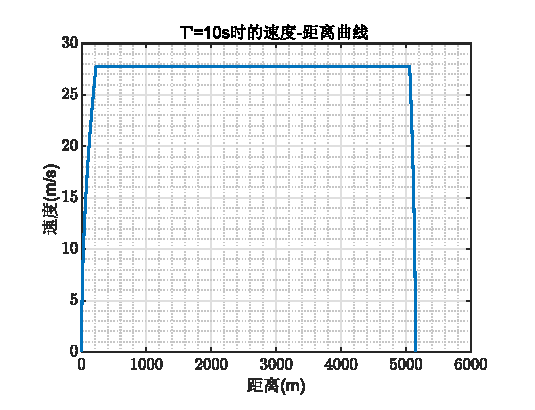
\includegraphics[width=.49\textwidth,height=0.3\textwidth]{figures/10a.eps}
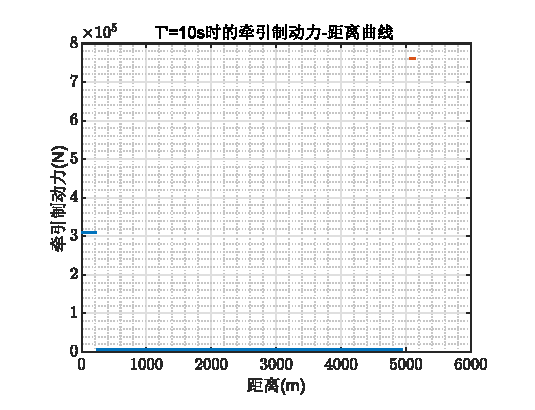
\includegraphics[width=.49\textwidth,height=0.3\textwidth]{figures/10b.eps}
\includegraphics[width=.49\textwidth,height=0.3\textwidth]{figures/10c.eps}
\includegraphics[width=.49\textwidth,height=0.3\textwidth]{figures/10d.eps}
\caption{\song\wuhao $T'=10s$时的曲线组}
\end{figure}
\begin{figure}[H]
\centering
\includegraphics[width=.49\textwidth,height=0.3\textwidth]{figures/20a.eps}
\includegraphics[width=.49\textwidth,height=0.3\textwidth]{figures/20b.eps}
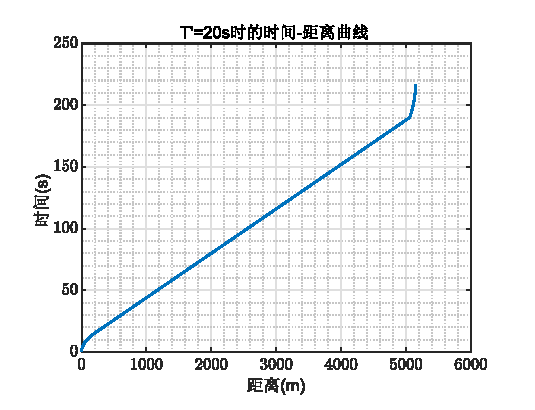
\includegraphics[width=.49\textwidth,height=0.3\textwidth]{figures/20c.eps}
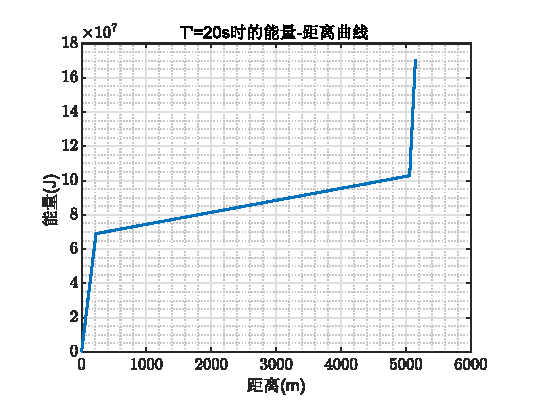
\includegraphics[width=.49\textwidth,height=0.3\textwidth]{figures/20d.eps}
\caption{\song\wuhao $T'=20s$时的曲线组}
\end{figure}
\begin{figure}[H]
\centering
\includegraphics[width=.49\textwidth,height=0.3\textwidth]{figures/50a.eps}
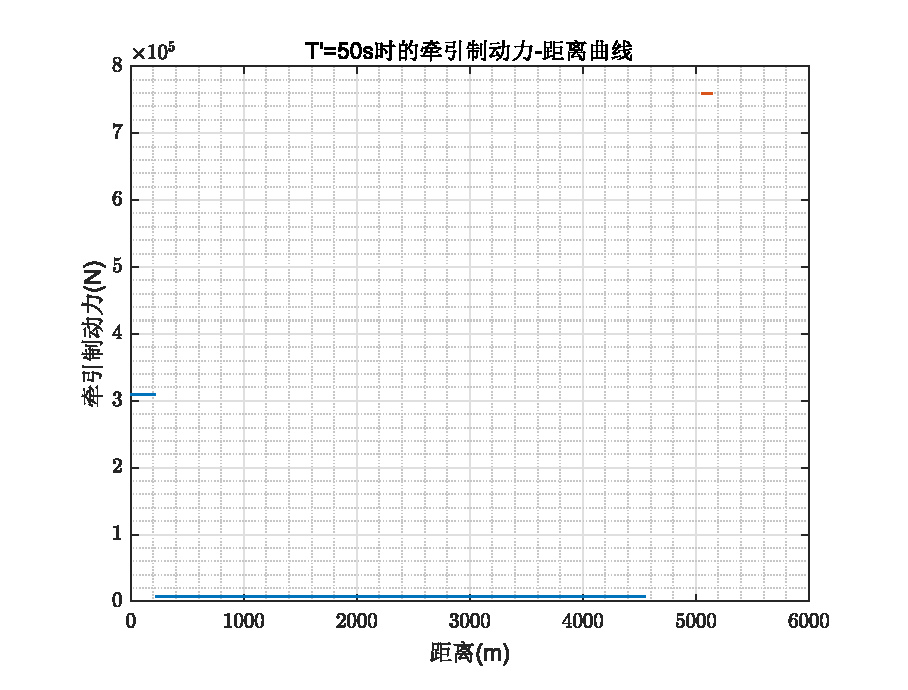
\includegraphics[width=.49\textwidth,height=0.3\textwidth]{figures/50b.eps}
\includegraphics[width=.49\textwidth,height=0.3\textwidth]{figures/50c.eps}
\includegraphics[width=.49\textwidth,height=0.3\textwidth]{figures/50d.eps}
\caption{\song\wuhao $T'=50s$时的曲线组}
\end{figure}
\begin{figure}[H]
\centering
\includegraphics[width=.49\textwidth,height=0.3\textwidth]{figures/150a.eps}
\includegraphics[width=.49\textwidth,height=0.3\textwidth]{figures/150b.eps}
\includegraphics[width=.49\textwidth,height=0.3\textwidth]{figures/150c.eps}
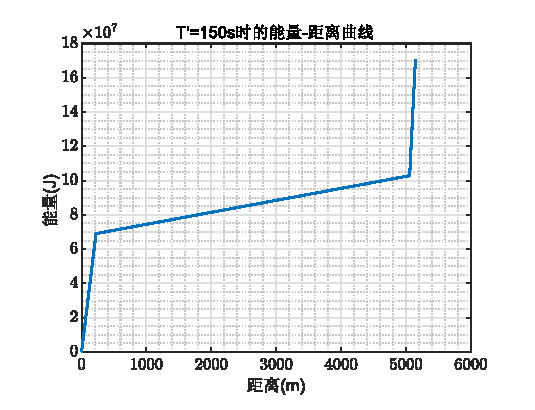
\includegraphics[width=.49\textwidth,height=0.3\textwidth]{figures/150d.eps}
\caption{\song\wuhao $T'=150s$时的曲线组}
\end{figure}
\begin{figure}[H]
\centering
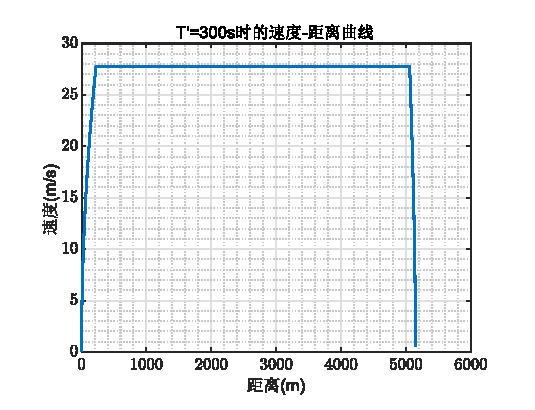
\includegraphics[width=.49\textwidth,height=0.3\textwidth]{figures/300a.eps}
\includegraphics[width=.49\textwidth,height=0.3\textwidth]{figures/300b.eps}
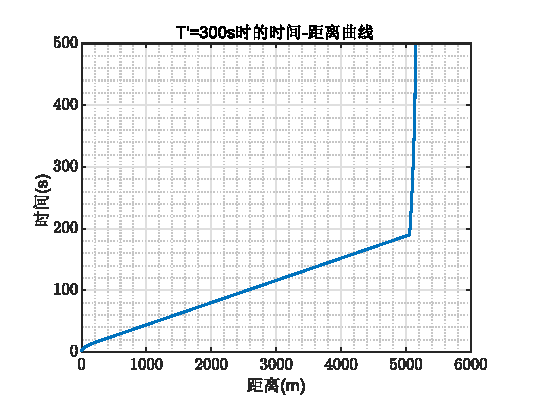
\includegraphics[width=.49\textwidth,height=0.3\textwidth]{figures/300c.eps}
\includegraphics[width=.49\textwidth,height=0.3\textwidth]{figures/300d.eps}
\caption{\song\wuhao $T'=300s$时的曲线组}
\end{figure}


























\section{问题二的模型建立与求解}
由于列车运行的不同道路段的最高限速和坡度都不完全相同,我们首先根据附件二中的路况信息可视化各路段的坡度和最大速度限制,再对不同道路段进行离散化处理,如图:
\begin{figure}[H]
\centering


\tikzset{every picture/.style={line width=0.75pt}} %set default line width to 0.75pt        

\begin{tikzpicture}[x=0.75pt,y=0.75pt,yscale=-1,xscale=1]
%uncomment if require: \path (0,488); %set diagram left start at 0, and has height of 488

%Image [id:dp9413694914413653] 
\draw (343.5,163.56) node  {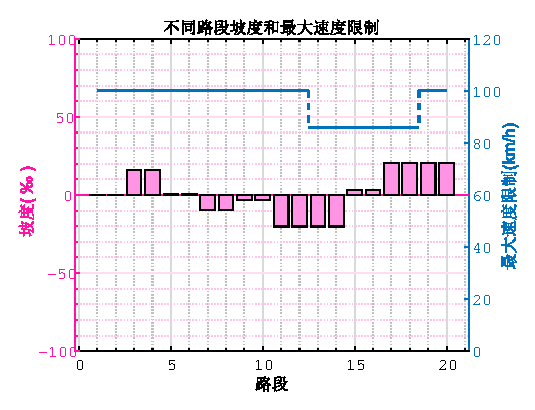
\includegraphics[width=338.26pt,height=246.85pt]{figures/e.eps}};
%Straight Lines [id:da49319795786838383] 
\draw [color={rgb, 255:red, 28; green, 220; blue, 248 }  ,draw opacity=1 ] [dash pattern={on 4.5pt off 4.5pt}]  (216.62,22.12) -- (216.62,291.12) ;
%Straight Lines [id:da18097750622320263] 
\draw [color={rgb, 255:red, 248; green, 231; blue, 28 }  ,draw opacity=1 ][line width=1.5]    (197.87,274) -- (174.74,331.34) ;
\draw [shift={(173.62,334.12)}, rotate = 291.97] [color={rgb, 255:red, 248; green, 231; blue, 28 }  ,draw opacity=1 ][line width=1.5]    (14.21,-4.28) .. controls (9.04,-1.82) and (4.3,-0.39) .. (0,0) .. controls (4.3,0.39) and (9.04,1.82) .. (14.21,4.28)   ;
%Straight Lines [id:da654182054182983] 
\draw [color={rgb, 255:red, 28; green, 220; blue, 248 }  ,draw opacity=1 ] [dash pattern={on 4.5pt off 4.5pt}]  (247.62,23.12) -- (247.62,292.12) ;
%Straight Lines [id:da2546948287499664] 
\draw [color={rgb, 255:red, 28; green, 220; blue, 248 }  ,draw opacity=1 ] [dash pattern={on 4.5pt off 4.5pt}]  (281.62,22.12) -- (281.62,291.12) ;
%Straight Lines [id:da17489154531806128] 
\draw [color={rgb, 255:red, 28; green, 220; blue, 248 }  ,draw opacity=1 ] [dash pattern={on 4.5pt off 4.5pt}]  (313.62,23.12) -- (313.62,292.12) ;
%Straight Lines [id:da6432434107909066] 
\draw [color={rgb, 255:red, 28; green, 220; blue, 248 }  ,draw opacity=1 ] [dash pattern={on 4.5pt off 4.5pt}]  (347.62,21.12) -- (347.62,290.12) ;
%Straight Lines [id:da47356853568303725] 
\draw [color={rgb, 255:red, 28; green, 220; blue, 248 }  ,draw opacity=1 ] [dash pattern={on 4.5pt off 4.5pt}]  (380.62,21.12) -- (380.62,290.12) ;
%Straight Lines [id:da9783690626751256] 
\draw [color={rgb, 255:red, 28; green, 220; blue, 248 }  ,draw opacity=1 ] [dash pattern={on 4.5pt off 4.5pt}]  (413.62,22.12) -- (413.62,291.12) ;
%Straight Lines [id:da8213769979349499] 
\draw [color={rgb, 255:red, 28; green, 220; blue, 248 }  ,draw opacity=1 ] [dash pattern={on 4.5pt off 4.5pt}]  (447.62,23.12) -- (447.62,292.12) ;
%Straight Lines [id:da3177911912601208] 
\draw [color={rgb, 255:red, 28; green, 220; blue, 248 }  ,draw opacity=1 ] [dash pattern={on 4.5pt off 4.5pt}]  (479.62,21.12) -- (479.62,290.12) ;
%Straight Lines [id:da3539263588655368] 
\draw [color={rgb, 255:red, 28; green, 220; blue, 248 }  ,draw opacity=1 ] [dash pattern={on 4.5pt off 4.5pt}]  (512.62,20.12) -- (512.62,289.12) ;
%Straight Lines [id:da995537290085831] 
\draw [color={rgb, 255:red, 248; green, 231; blue, 28 }  ,draw opacity=1 ][line width=1.5]    (235.87,273) -- (215.67,346.11) ;
\draw [shift={(214.87,349)}, rotate = 285.45] [color={rgb, 255:red, 248; green, 231; blue, 28 }  ,draw opacity=1 ][line width=1.5]    (14.21,-4.28) .. controls (9.04,-1.82) and (4.3,-0.39) .. (0,0) .. controls (4.3,0.39) and (9.04,1.82) .. (14.21,4.28)   ;
%Straight Lines [id:da972202227698985] 
\draw [color={rgb, 255:red, 248; green, 231; blue, 28 }  ,draw opacity=1 ][line width=1.5]    (502.62,267.62) -- (513.45,344.03) ;
\draw [shift={(513.87,347)}, rotate = 261.93] [color={rgb, 255:red, 248; green, 231; blue, 28 }  ,draw opacity=1 ][line width=1.5]    (14.21,-4.28) .. controls (9.04,-1.82) and (4.3,-0.39) .. (0,0) .. controls (4.3,0.39) and (9.04,1.82) .. (14.21,4.28)   ;
%Straight Lines [id:da9372396633623898] 
\draw [color={rgb, 255:red, 0; green, 0; blue, 0 }  ,draw opacity=1 ][line width=1.5]  [dash pattern={on 0.75pt off 2.25pt}]  (262.87,365.99) -- (468.87,365.02) ;
\draw [shift={(472.87,365)}, rotate = 179.73] [fill={rgb, 255:red, 0; green, 0; blue, 0 }  ,fill opacity=1 ][line width=0.08]  [draw opacity=0] (13.4,-6.43) -- (0,0) -- (13.4,6.44) -- (8.9,0) -- cycle    ;
\draw [shift={(258.87,366)}, rotate = 359.73] [fill={rgb, 255:red, 0; green, 0; blue, 0 }  ,fill opacity=1 ][line width=0.08]  [draw opacity=0] (13.4,-6.43) -- (0,0) -- (13.4,6.44) -- (8.9,0) -- cycle    ;

% Text Node
\draw (142,345) node [anchor=north west][inner sep=0.75pt]  [color={rgb, 255:red, 0; green, 0; blue, 0 }  ,opacity=1 ] [align=left] {路段1};
% Text Node
\draw (187,358.5) node [anchor=north west][inner sep=0.75pt]  [color={rgb, 255:red, 0; green, 0; blue, 0 }  ,opacity=1 ] [align=left] {路段2};
% Text Node
\draw (487,355.5) node [anchor=north west][inner sep=0.75pt]  [color={rgb, 255:red, 0; green, 0; blue, 0 }  ,opacity=1 ] [align=left] {路段10};


\end{tikzpicture}

\caption{\song\wuhao 路段的划分}
\end{figure}

我们首先假设线路$X$由$n$个不同的离散区间$X_n$组成,满足:
\begin{eqnarray}
{\textstyle \bigcup\limits_{n}}X_n=X \quad \& \quad {\textstyle \bigcap\limits_{n}}X_n=\emptyset
\end{eqnarray}

使得线路中各个区间的优化目标下列车的能耗为$E_X$,则有:
\begin{eqnarray}
E_X=\min\sum\limits_{i=1}^nE_{X_n}
\end{eqnarray}

我们容易得到的约束条件有:
\begin{eqnarray}
0\le v_{X_n}\le v_{{X_n}_{max}}
\end{eqnarray}

列车在坡道中所受到的重力也会阻碍列车前进,有:
\begin{eqnarray}
F_\theta =mg\sin\theta
\end{eqnarray}

所以坡道单位阻力有:
\begin{eqnarray}
f_\theta=\frac{F_\theta}{mg}=\sin\theta
\end{eqnarray}

由于坡道中没有出现大于$30\textperthousand$ 的坡度$\theta$ ,所以我们可以近似认为$\sin\theta=\theta$,则有:
\begin{eqnarray}
f_\theta=\theta
\end{eqnarray}
其中,$f_\theta$为坡度为$\theta$时的坡道阻力。

我们的列车线路区间的部分参数如表所示:
\begin{table}[H]
\centering
\caption{各离散线路区间部分参数}
\label{bh}
\begin{tabular}{ccccc}
\hline
\textbf{线路编号} & \textbf{起点位置/m} & \textbf{终点位置/m} & \textbf{坡度/‰} & \textbf{限速/(km/h)} \\ \hline
路段1           & 0               & 198.967         & 0.0617284     & 100                \\
路段2           & 198.967         & 739.018         & 16.2346       & 100                \\
路段3           & 739.018         & 2217.05         & 0.679012      & 100                \\
路段4           & 2217.05         & 2870.8          & -9.81481      & 100                \\
路段5           & 2870.8          & 4178.29         & -3.02469      & 100                \\
路段6           & 4178.29         & 4259.1          & -20.1852      & 100                \\
路段7           & 4259.1          & 4604.66         & -20.1852      & 86                 \\
路段8           & 4604.66         & 4803.63         & 3.02469       & 86                 \\
路段9           & 4803.63         & 4960.1          & 20.3086       & 86                 \\
路段10          & 4960.1          & 5144.7          & 20.3086       & 100                \\ \hline
\end{tabular}
\end{table}

根据线路数据,通过离散化理论建立消耗能量-时间的对应关系,利用基于栅格模型的蚁群算法,求解各离散的线路区间速度的最优解,该算法流程图展示在图\ref{lct}中,求得的列车最优速度曲线如图\ref{zuiyou}:
\begin{figure}
\centering
\includegraphics[scale=0.3]{figures/diagram-20230513.png}
\caption{基于栅格模型的蚁群算法流程图}\label{lct}
\end{figure}


\begin{figure}[H]
\centering
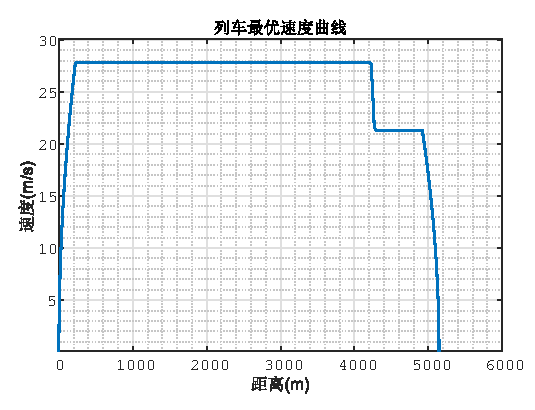
\includegraphics{figures/zysd.eps}
\caption{列车最优速度曲线}\label{zuiyou}
\end{figure}

考虑最短运行时间的列车运行时间,容易发现应当让列车在最大限速运行的时间最长,我们做出列车$v$-$t$图像如图所示:
\begin{figure}[H]
\centering
\tikzset{every picture/.style={line width=0.75pt}} %set default line width to 0.75pt        

\begin{tikzpicture}[x=0.75pt,y=0.75pt,yscale=-1,xscale=1]
%uncomment if require: \path (0,300); %set diagram left start at 0, and has height of 300

%Straight Lines [id:da0857601338659093] 
\draw    (99.99,210.06) -- (100.48,31.06) ;
\draw [shift={(100.49,29.06)}, rotate = 90.16] [color={rgb, 255:red, 0; green, 0; blue, 0 }  ][line width=0.75]    (10.93,-3.29) .. controls (6.95,-1.4) and (3.31,-0.3) .. (0,0) .. controls (3.31,0.3) and (6.95,1.4) .. (10.93,3.29)   ;
%Straight Lines [id:da45900269236989355] 
\draw    (99.99,210.06) -- (399.06,210.62) ;
\draw [shift={(401.06,210.63)}, rotate = 180.11] [color={rgb, 255:red, 0; green, 0; blue, 0 }  ][line width=0.75]    (10.93,-3.29) .. controls (6.95,-1.4) and (3.31,-0.3) .. (0,0) .. controls (3.31,0.3) and (6.95,1.4) .. (10.93,3.29)   ;
%Curve Lines [id:da6769226143475053] 
\draw    (99.99,210.06) .. controls (98.49,169.06) and (107.99,129.06) .. (147.99,99.06) ;
%Straight Lines [id:da8144378967631352] 
\draw    (147.99,99.06) -- (230.99,99.56) ;
%Curve Lines [id:da471463763752624] 
\draw    (230.99,99.56) .. controls (231.56,110.13) and (231.06,140.13) .. (235.06,140.63) ;
%Straight Lines [id:da49592969387578334] 
\draw    (235.06,140.63) -- (309.99,140.06) ;
%Curve Lines [id:da8031471501192691] 
\draw    (309.99,140.06) .. controls (312.49,214.56) and (365.56,207.63) .. (365.06,210.63) ;
%Straight Lines [id:da3454940306346235] 
\draw  [dash pattern={on 0.84pt off 2.51pt}]  (147.99,99.06) -- (100.49,99.06) ;
%Straight Lines [id:da10794886512335267] 
\draw  [dash pattern={on 0.84pt off 2.51pt}]  (100,140.13) -- (235.06,140.63) ;
%Straight Lines [id:da22635356681537067] 
\draw  [dash pattern={on 0.84pt off 2.51pt}]  (147.99,99.06) -- (147.56,209.63) ;
%Straight Lines [id:da45430378888531964] 
\draw  [dash pattern={on 0.84pt off 2.51pt}]  (230.99,99.56) -- (230.38,171.62) -- (230.06,210.13) ;
%Straight Lines [id:da7957669804465681] 
\draw  [dash pattern={on 0.84pt off 2.51pt}]  (309.99,140.06) -- (309.56,209.63) ;
%Straight Lines [id:da7125741346341208] 
\draw  [dash pattern={on 0.84pt off 2.51pt}]  (235.06,140.63) -- (234.64,210.19) ;

% Text Node
\draw (67.36,89) node [anchor=north west][inner sep=0.75pt]   [align=left] {$\displaystyle v_{max}$};
% Text Node
\draw (67,131.5) node [anchor=north west][inner sep=0.75pt]   [align=left] {$\displaystyle v'_{max}$};
% Text Node
\draw (140.5,212) node [anchor=north west][inner sep=0.75pt]   [align=left] {$\displaystyle t_{0}$};
% Text Node
\draw (88.5,33) node [anchor=north west][inner sep=0.75pt]   [align=left] {$\displaystyle v$};
% Text Node
\draw (388.5,213.5) node [anchor=north west][inner sep=0.75pt]   [align=left] {$\displaystyle t$};
% Text Node
\draw (214.5,212.5) node [anchor=north west][inner sep=0.75pt]   [align=left] {$\displaystyle t_{1}$};
% Text Node
\draw (302,212.5) node [anchor=north west][inner sep=0.75pt]   [align=left] {$\displaystyle t_{3}$};
% Text Node
\draw (236.64,213.19) node [anchor=north west][inner sep=0.75pt]   [align=left] {$\displaystyle t_{2}$};
% Text Node
\draw (357.5,212.5) node [anchor=north west][inner sep=0.75pt]   [align=left] {$\displaystyle T$};


\end{tikzpicture}
\caption{考虑路况情况下最短时间的$v$-$t$曲线}
\end{figure}

我们再列出微分方程利用龙格库塔算法进行求解并画图如下:
\begin{figure}[H]
\centering
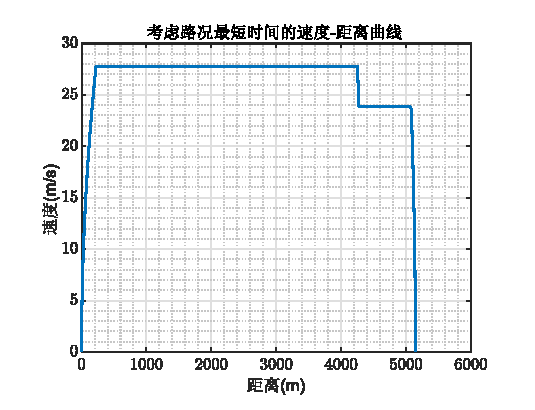
\includegraphics[width=.49\textwidth]{figures/aa.eps}
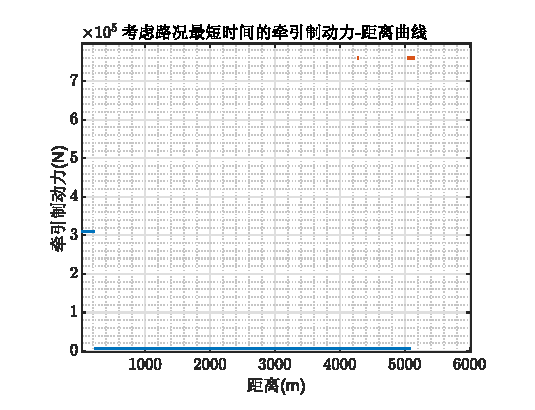
\includegraphics[width=.49\textwidth]{figures/bb.eps}
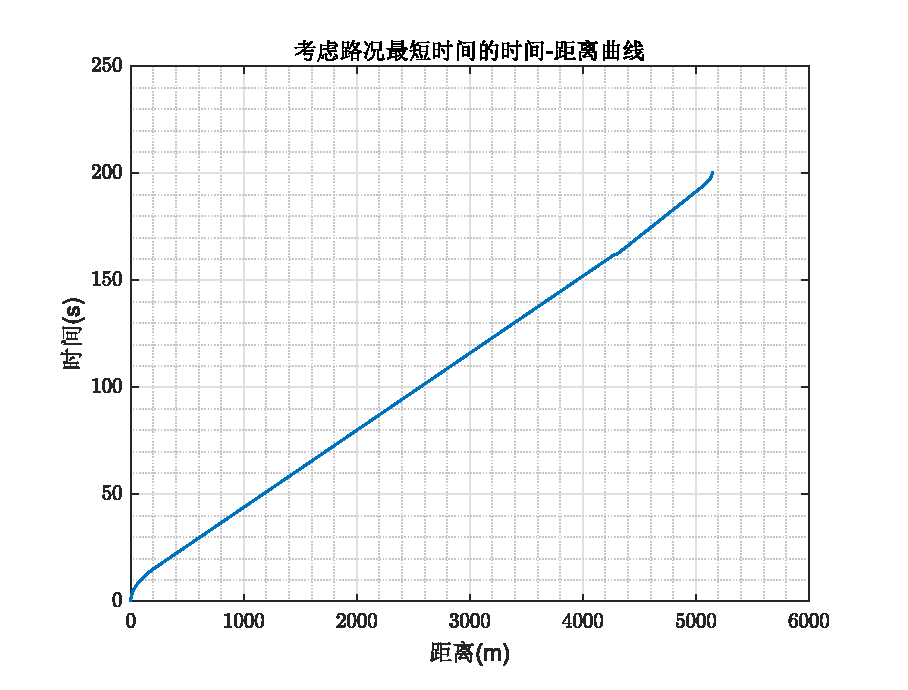
\includegraphics[width=.49\textwidth]{figures/cc.eps}
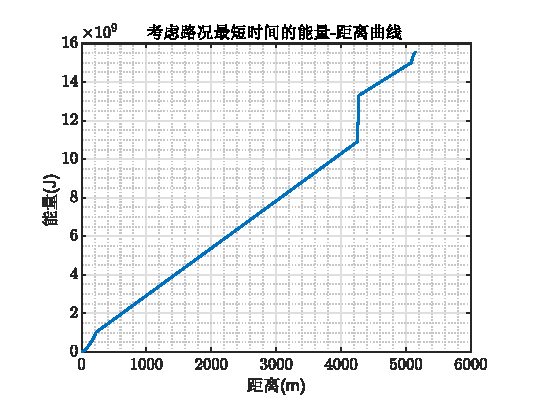
\includegraphics[width=.49\textwidth]{figures/dd.eps}
\caption{\song\wuhao 考虑路况情况下最短时间的曲线组}
\end{figure}



在最短时间上增加时间$T'$,我们考虑列车在最后减速阶段前进入惰行阶段,示意图如图\ref{dxdx}所示,这样我们就得到了不同$T'$的曲线组如下:
\begin{figure}[H]
\centering
\resizebox{\textwidth}{!}{
\tikzset{every picture/.style={line width=0.75pt}} %set default line width to 0.75pt        

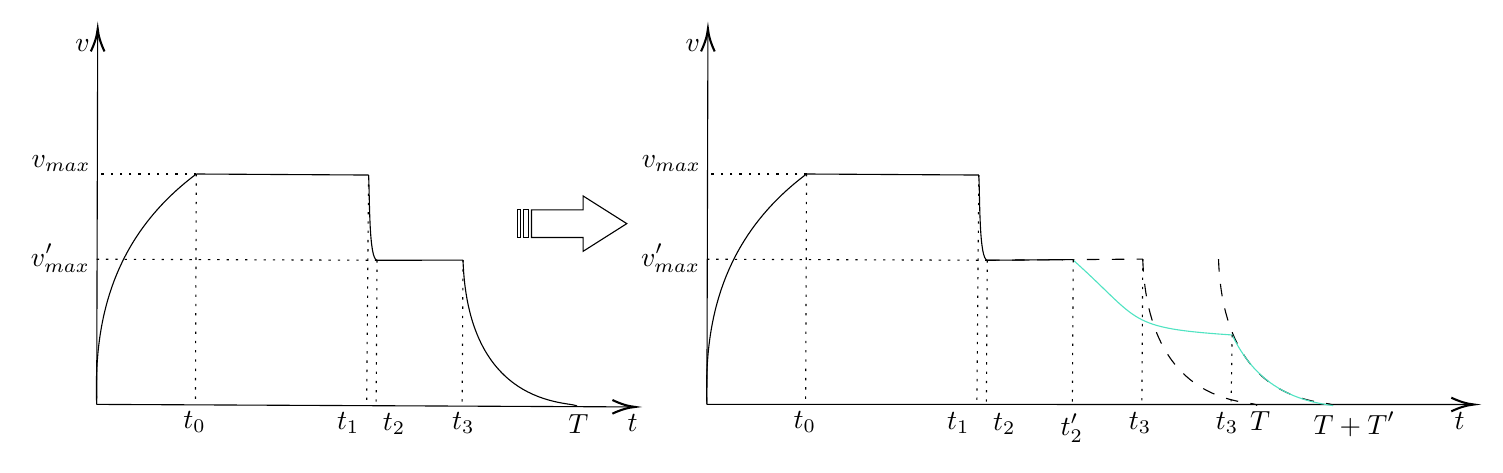
\begin{tikzpicture}[x=0.75pt,y=0.75pt,yscale=-1,xscale=1]
%uncomment if require: \path (0,300); %set diagram left start at 0, and has height of 300

%Straight Lines [id:da0857601338659093] 
\draw    (328.65,199.4) -- (329.15,20.4) ;
\draw [shift={(329.15,18.4)}, rotate = 90.16] [color={rgb, 255:red, 0; green, 0; blue, 0 }  ][line width=0.75]    (10.93,-3.29) .. controls (6.95,-1.4) and (3.31,-0.3) .. (0,0) .. controls (3.31,0.3) and (6.95,1.4) .. (10.93,3.29)   ;
%Straight Lines [id:da45900269236989355] 
\draw    (328.65,199.4) -- (696.23,199.46) ;
\draw [shift={(698.23,199.46)}, rotate = 180.01] [color={rgb, 255:red, 0; green, 0; blue, 0 }  ][line width=0.75]    (10.93,-3.29) .. controls (6.95,-1.4) and (3.31,-0.3) .. (0,0) .. controls (3.31,0.3) and (6.95,1.4) .. (10.93,3.29)   ;
%Curve Lines [id:da6769226143475053] 
\draw    (328.65,199.4) .. controls (327.15,158.4) and (336.65,118.4) .. (376.65,88.4) ;
%Straight Lines [id:da8144378967631352] 
\draw    (376.65,88.4) -- (459.65,88.9) ;
%Curve Lines [id:da471463763752624] 
\draw    (459.65,88.9) .. controls (460.23,99.46) and (459.73,129.46) .. (463.73,129.96) ;
%Straight Lines [id:da49592969387578334] 
\draw  [dash pattern={on 4.5pt off 4.5pt}]  (463.73,129.96) -- (538.65,129.4) ;
%Curve Lines [id:da8031471501192691] 
\draw  [dash pattern={on 4.5pt off 4.5pt}]  (538.65,129.4) .. controls (541.15,203.9) and (594.23,196.96) .. (593.73,199.96) ;
%Straight Lines [id:da3454940306346235] 
\draw  [dash pattern={on 0.84pt off 2.51pt}]  (376.65,88.4) -- (329.15,88.4) ;
%Straight Lines [id:da10794886512335267] 
\draw  [dash pattern={on 0.84pt off 2.51pt}]  (328.67,129.46) -- (463.73,129.96) ;
%Straight Lines [id:da22635356681537067] 
\draw  [dash pattern={on 0.84pt off 2.51pt}]  (376.65,88.4) -- (376.23,198.96) ;
%Straight Lines [id:da45430378888531964] 
\draw  [dash pattern={on 0.84pt off 2.51pt}]  (459.65,88.9) -- (459.05,160.95) -- (458.73,199.46) ;
%Straight Lines [id:da7957669804465681] 
\draw  [dash pattern={on 0.84pt off 2.51pt}]  (538.65,129.4) -- (538.23,198.96) ;
%Straight Lines [id:da7125741346341208] 
\draw  [dash pattern={on 0.84pt off 2.51pt}]  (463.73,129.96) -- (463.3,199.52) ;
%Straight Lines [id:da43024150385457305] 
\draw    (463.73,129.96) -- (501.19,129.68) ;
%Curve Lines [id:da5300333508708877] 
\draw  [dash pattern={on 4.5pt off 4.5pt}]  (575.15,129.4) .. controls (575.53,140.74) and (577.09,150.2) .. (579.45,158.1) .. controls (592.58,202.01) and (630.65,197.42) .. (630.23,199.96) ;
%Curve Lines [id:da011942953949924062] 
\draw [color={rgb, 255:red, 80; green, 227; blue, 194 }  ,draw opacity=1 ]   (505.15,129.9) .. controls (538.23,159.46) and (530.23,162.46) .. (581.73,165.96) ;
%Straight Lines [id:da5973962001157187] 
\draw  [dash pattern={on 0.84pt off 2.51pt}]  (505.15,129.9) -- (504.73,199.46) ;
%Curve Lines [id:da5066432510896688] 
\draw [color={rgb, 255:red, 80; green, 227; blue, 194 }  ,draw opacity=1 ]   (581.73,165.96) .. controls (583.55,169.77) and (585.55,173.17) .. (587.68,176.2) .. controls (588.65,177.57) and (589.64,178.87) .. (590.67,180.09) .. controls (601.6,193.16) and (615.62,198.04) .. (630.23,199.96) ;
%Straight Lines [id:da4599773406537844] 
\draw  [dash pattern={on 0.84pt off 2.51pt}]  (581.73,165.96) -- (581.57,175.97) -- (581.23,197.96) ;
%Straight Lines [id:da8390869226690223] 
\draw    (34.65,199.4) -- (35.15,20.4) ;
\draw [shift={(35.15,18.4)}, rotate = 90.16] [color={rgb, 255:red, 0; green, 0; blue, 0 }  ][line width=0.75]    (10.93,-3.29) .. controls (6.95,-1.4) and (3.31,-0.3) .. (0,0) .. controls (3.31,0.3) and (6.95,1.4) .. (10.93,3.29)   ;
%Straight Lines [id:da6424697016343339] 
\draw    (34.65,199.4) -- (292.06,200.62) ;
\draw [shift={(294.06,200.63)}, rotate = 180.27] [color={rgb, 255:red, 0; green, 0; blue, 0 }  ][line width=0.75]    (10.93,-3.29) .. controls (6.95,-1.4) and (3.31,-0.3) .. (0,0) .. controls (3.31,0.3) and (6.95,1.4) .. (10.93,3.29)   ;
%Curve Lines [id:da4159520979982092] 
\draw    (34.65,199.4) .. controls (33.15,158.4) and (42.65,118.4) .. (82.65,88.4) ;
%Straight Lines [id:da7397065699883372] 
\draw    (82.65,88.4) -- (165.65,88.9) ;
%Curve Lines [id:da5542327588280489] 
\draw    (165.65,88.9) .. controls (166.23,99.46) and (165.73,129.46) .. (169.73,129.96) ;
%Curve Lines [id:da9512778770596777] 
\draw    (211.15,129.9) .. controls (213.65,204.4) and (266.73,197.46) .. (266.23,200.46) ;
%Straight Lines [id:da7867883976550687] 
\draw  [dash pattern={on 0.84pt off 2.51pt}]  (82.65,88.4) -- (35.15,88.4) ;
%Straight Lines [id:da737867179342663] 
\draw  [dash pattern={on 0.84pt off 2.51pt}]  (34.67,129.46) -- (169.73,129.96) ;
%Straight Lines [id:da9221487760657978] 
\draw  [dash pattern={on 0.84pt off 2.51pt}]  (82.65,88.4) -- (82.23,198.96) ;
%Straight Lines [id:da8264008180595217] 
\draw  [dash pattern={on 0.84pt off 2.51pt}]  (165.65,88.9) -- (165.05,160.95) -- (164.73,199.46) ;
%Straight Lines [id:da4418859502549326] 
\draw  [dash pattern={on 0.84pt off 2.51pt}]  (169.73,129.96) -- (169.3,199.52) ;
%Straight Lines [id:da921188263298494] 
\draw    (169.73,129.96) -- (211.15,129.9) ;
%Straight Lines [id:da25401914347911525] 
\draw  [dash pattern={on 0.84pt off 2.51pt}]  (211.15,129.9) -- (210.73,199.46) ;
%Striped Right Arrow [id:dp428339183673732] 
\draw   (244.16,105.66) -- (269.04,105.66) -- (269.04,99) -- (290.06,112.31) -- (269.04,125.63) -- (269.04,118.97) -- (244.16,118.97) -- cycle ;\draw   (237.5,105.66) -- (238.83,105.66) -- (238.83,118.97) -- (237.5,118.97) -- cycle ;\draw   (240.16,105.66) -- (242.83,105.66) -- (242.83,118.97) -- (240.16,118.97) -- cycle ;

% Text Node
\draw (296.03,78.33) node [anchor=north west][inner sep=0.75pt]   [align=left] {$\displaystyle v_{max}$};
% Text Node
\draw (295.67,120.83) node [anchor=north west][inner sep=0.75pt]   [align=left] {$\displaystyle v'_{max}$};
% Text Node
\draw (369.17,201.33) node [anchor=north west][inner sep=0.75pt]   [align=left] {$\displaystyle t_{0}$};
% Text Node
\draw (317.17,22.33) node [anchor=north west][inner sep=0.75pt]   [align=left] {$\displaystyle v$};
% Text Node
\draw (687.67,201.83) node [anchor=north west][inner sep=0.75pt]   [align=left] {$\displaystyle t$};
% Text Node
\draw (443.17,201.83) node [anchor=north west][inner sep=0.75pt]   [align=left] {$\displaystyle t_{1}$};
% Text Node
\draw (530.67,201.83) node [anchor=north west][inner sep=0.75pt]   [align=left] {$\displaystyle t_{3}$};
% Text Node
\draw (465.3,202.52) node [anchor=north west][inner sep=0.75pt]   [align=left] {$\displaystyle t_{2}$};
% Text Node
\draw (497.8,202.52) node [anchor=north west][inner sep=0.75pt]   [align=left] {$\displaystyle t'_{2}$};
% Text Node
\draw (572.67,201.83) node [anchor=north west][inner sep=0.75pt]   [align=left] {$\displaystyle t_{3}$};
% Text Node
\draw (589.17,201.83) node [anchor=north west][inner sep=0.75pt]   [align=left] {$\displaystyle T$};
% Text Node
\draw (619.67,201.83) node [anchor=north west][inner sep=0.75pt]   [align=left] {$\displaystyle T+T'$};
% Text Node
\draw (2.03,78.33) node [anchor=north west][inner sep=0.75pt]   [align=left] {$\displaystyle v_{max}$};
% Text Node
\draw (1.67,120.83) node [anchor=north west][inner sep=0.75pt]   [align=left] {$\displaystyle v'_{max}$};
% Text Node
\draw (75.17,201.33) node [anchor=north west][inner sep=0.75pt]   [align=left] {$\displaystyle t_{0}$};
% Text Node
\draw (23.17,22.33) node [anchor=north west][inner sep=0.75pt]   [align=left] {$\displaystyle v$};
% Text Node
\draw (289.17,202.83) node [anchor=north west][inner sep=0.75pt]   [align=left] {$\displaystyle t$};
% Text Node
\draw (149.17,201.83) node [anchor=north west][inner sep=0.75pt]   [align=left] {$\displaystyle t_{1}$};
% Text Node
\draw (204.67,201.83) node [anchor=north west][inner sep=0.75pt]   [align=left] {$\displaystyle t_{3}$};
% Text Node
\draw (171.3,202.52) node [anchor=north west][inner sep=0.75pt]   [align=left] {$\displaystyle t_{2}$};
% Text Node
\draw (260.67,202.83) node [anchor=north west][inner sep=0.75pt]   [align=left] {$\displaystyle T$};


\end{tikzpicture}}

\caption{考虑路况情况最短时间上增加时间$T'$时间的$v$-$t$曲线}\label{dxdx}
\end{figure}
\begin{figure}[H]
\centering
\includegraphics[width=.49\textwidth,height=0.3\textwidth]{figures/10aa.eps}
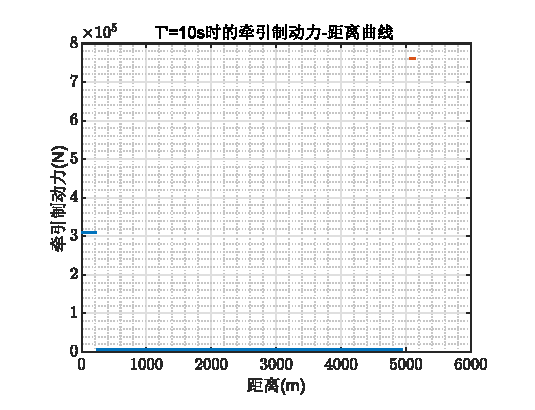
\includegraphics[width=.49\textwidth,height=0.3\textwidth]{figures/10b.eps}
\includegraphics[width=.49\textwidth,height=0.3\textwidth]{figures/10cc.eps}
\includegraphics[width=.49\textwidth,height=0.3\textwidth]{figures/10dd.eps}
\caption{\song\wuhao 考虑路况情况下$T'=10s$时的曲线组}
\end{figure}
\begin{figure}[H]
\centering
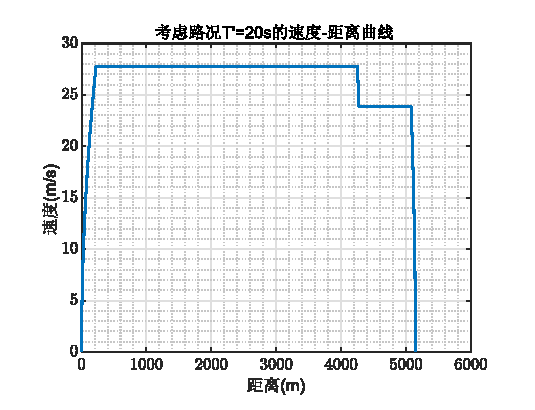
\includegraphics[width=.49\textwidth,height=0.3\textwidth]{figures/20aa.eps}
\includegraphics[width=.49\textwidth,height=0.3\textwidth]{figures/20bb.eps}
\includegraphics[width=.49\textwidth,height=0.3\textwidth]{figures/20cc.eps}
\includegraphics[width=.49\textwidth,height=0.3\textwidth]{figures/20dd.eps}
\caption{\song\wuhao 考虑路况情况下$T'=20s$时的曲线组}
\end{figure}
\begin{figure}[H]
\centering
\includegraphics[width=.49\textwidth,height=0.3\textwidth]{figures/50aa.eps}
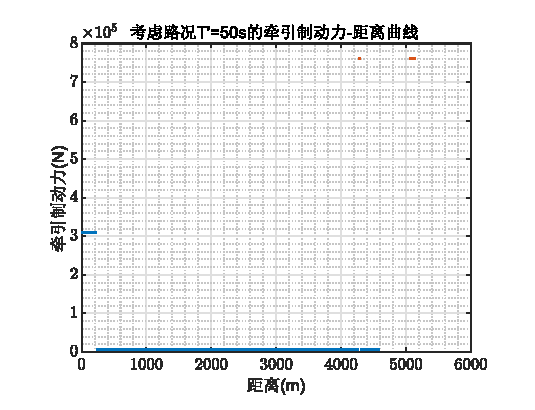
\includegraphics[width=.49\textwidth,height=0.3\textwidth]{figures/50bb.eps}
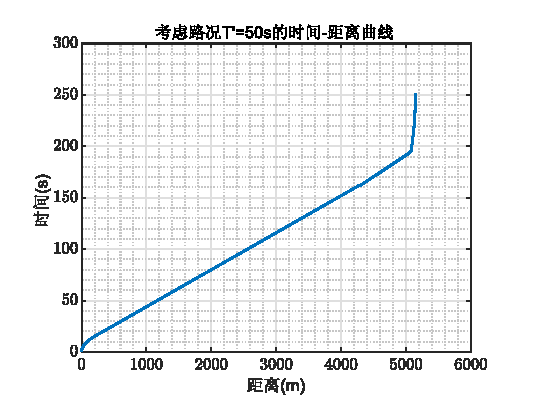
\includegraphics[width=.49\textwidth,height=0.3\textwidth]{figures/50cc.eps}
\includegraphics[width=.49\textwidth,height=0.3\textwidth]{figures/50dd.eps}
\caption{\song\wuhao 考虑路况情况下$T'=50s$时的曲线组}
\end{figure}
\begin{figure}[H]
\centering
\includegraphics[width=.49\textwidth,height=0.3\textwidth]{figures/150aa.eps}
\includegraphics[width=.49\textwidth,height=0.3\textwidth]{figures/150bb.eps}
\includegraphics[width=.49\textwidth,height=0.3\textwidth]{figures/150cc.eps}
\includegraphics[width=.49\textwidth,height=0.3\textwidth]{figures/150dd.eps}
\caption{\song\wuhao 考虑路况情况下$T'=150s$时的曲线组}
\end{figure}
\begin{figure}[H]
\centering
\includegraphics[width=.49\textwidth,height=0.3\textwidth]{figures/300aa.eps}
\includegraphics[width=.49\textwidth,height=0.3\textwidth]{figures/300bb.eps}
\includegraphics[width=.49\textwidth,height=0.3\textwidth]{figures/300cc.eps}
\includegraphics[width=.49\textwidth,height=0.3\textwidth]{figures/300dd.eps}
\caption{\song\wuhao 考虑路况情况下$T'=300s$时的曲线组}
\end{figure}






































% \tikzset{every picture/.style={line width=0.75pt}} %set default line width to 0.75pt        

% \begin{tikzpicture}[x=0.75pt,y=0.75pt,yscale=-1,xscale=1]
% %uncomment if require: \path (0,300); %set diagram left start at 0, and has height of 300

% %Flowchart: Process [id:dp10315671424148154] 
% \draw   (250.87,96) -- (369,96) -- (369,166) -- (250.87,166) -- cycle ;
% %Straight Lines [id:da647077685385115] 
% \draw    (309.94,131) -- (448.38,130.67) ;
% \draw [shift={(450.38,130.66)}, rotate = 179.86] [color={rgb, 255:red, 0; green, 0; blue, 0 }  ][line width=0.75]    (10.93,-3.29) .. controls (6.95,-1.4) and (3.31,-0.3) .. (0,0) .. controls (3.31,0.3) and (6.95,1.4) .. (10.93,3.29)   ;
% \draw [shift={(309.94,131)}, rotate = 359.86] [color={rgb, 255:red, 0; green, 0; blue, 0 }  ][fill={rgb, 255:red, 0; green, 0; blue, 0 }  ][line width=0.75]      (0, 0) circle [x radius= 3.35, y radius= 3.35]   ;
% %Straight Lines [id:da2808625059085279] 
% \draw    (309.94,131) -- (212.79,130.63) -- (212.38,130.63) ;
% \draw [shift={(210.38,130.66)}, rotate = 359.22] [color={rgb, 255:red, 0; green, 0; blue, 0 }  ][line width=0.75]    (10.93,-3.29) .. controls (6.95,-1.4) and (3.31,-0.3) .. (0,0) .. controls (3.31,0.3) and (6.95,1.4) .. (10.93,3.29)   ;
% %Straight Lines [id:da16427279858828814] 
% \draw    (287.58,86.26) -- (337.18,86.26) ;
% \draw [shift={(339.18,86.26)}, rotate = 180] [color={rgb, 255:red, 0; green, 0; blue, 0 }  ][line width=0.75]    (10.93,-3.29) .. controls (6.95,-1.4) and (3.31,-0.3) .. (0,0) .. controls (3.31,0.3) and (6.95,1.4) .. (10.93,3.29)   ;

% % Text Node
% \draw (433.59,141.47) node [anchor=north west][inner sep=0.75pt]   [align=left] {$\displaystyle F_{Q}$};
% % Text Node
% \draw (212.38,133.66) node [anchor=north west][inner sep=0.75pt]   [align=left] {$\displaystyle f$};
% % Text Node
% \draw (317.77,66.27) node [anchor=north west][inner sep=0.75pt]   [align=left] {$\displaystyle a$};
% % Text Node
% \draw (252.87,99) node [anchor=north west][inner sep=0.75pt]   [align=left] {$\displaystyle m$};


% \end{tikzpicture}



% \tikzset{every picture/.style={line width=0.75pt}} %set default line width to 0.75pt        

% \begin{tikzpicture}[x=0.75pt,y=0.75pt,yscale=-1,xscale=1]
% %uncomment if require: \path (0,300); %set diagram left start at 0, and has height of 300

% %Flowchart: Process [id:dp10315671424148154] 
% \draw   (250.87,96) -- (369,96) -- (369,166) -- (250.87,166) -- cycle ;
% %Straight Lines [id:da647077685385115] 
% \draw    (309.94,131) -- (447.39,130.8) ;
% \draw [shift={(449.39,130.8)}, rotate = 179.92] [color={rgb, 255:red, 0; green, 0; blue, 0 }  ][line width=0.75]    (10.93,-3.29) .. controls (6.95,-1.4) and (3.31,-0.3) .. (0,0) .. controls (3.31,0.3) and (6.95,1.4) .. (10.93,3.29)   ;
% \draw [shift={(309.94,131)}, rotate = 359.92] [color={rgb, 255:red, 0; green, 0; blue, 0 }  ][fill={rgb, 255:red, 0; green, 0; blue, 0 }  ][line width=0.75]      (0, 0) circle [x radius= 3.35, y radius= 3.35]   ;
% %Straight Lines [id:da2808625059085279] 
% \draw    (309.94,131) -- (172.39,130.47) ;
% \draw [shift={(170.39,130.47)}, rotate = 0.22] [color={rgb, 255:red, 0; green, 0; blue, 0 }  ][line width=0.75]    (10.93,-3.29) .. controls (6.95,-1.4) and (3.31,-0.3) .. (0,0) .. controls (3.31,0.3) and (6.95,1.4) .. (10.93,3.29)   ;

% % Text Node
% \draw (427.1,134.67) node [anchor=north west][inner sep=0.75pt]   [align=left] {$\displaystyle F_{Q}$};
% % Text Node
% \draw (172.39,133.47) node [anchor=north west][inner sep=0.75pt]   [align=left] {$\displaystyle f$};
% % Text Node
% \draw (287.38,74.67) node [anchor=north west][inner sep=0.75pt]   [align=left] {$\displaystyle a=0$};
% % Text Node
% \draw (252.87,99) node [anchor=north west][inner sep=0.75pt]   [align=left] {$\displaystyle m$};


% \end{tikzpicture}


% \tikzset{every picture/.style={line width=0.75pt}} %set default line width to 0.75pt        

% \begin{tikzpicture}[x=0.75pt,y=0.75pt,yscale=-1,xscale=1]
% %uncomment if require: \path (0,300); %set diagram left start at 0, and has height of 300

% %Flowchart: Process [id:dp10315671424148154] 
% \draw   (250.87,96) -- (369,96) -- (369,166) -- (250.87,166) -- cycle ;
% %Straight Lines [id:da647077685385115] 
% \draw    (309.94,131) -- (207.98,130.67) ;
% \draw [shift={(205.98,130.66)}, rotate = 0.19] [color={rgb, 255:red, 0; green, 0; blue, 0 }  ][line width=0.75]    (10.93,-3.29) .. controls (6.95,-1.4) and (3.31,-0.3) .. (0,0) .. controls (3.31,0.3) and (6.95,1.4) .. (10.93,3.29)   ;
% \draw [shift={(309.94,131)}, rotate = 180.19] [color={rgb, 255:red, 0; green, 0; blue, 0 }  ][fill={rgb, 255:red, 0; green, 0; blue, 0 }  ][line width=0.75]      (0, 0) circle [x radius= 3.35, y radius= 3.35]   ;
% %Straight Lines [id:da2808625059085279] 
% \draw    (309.94,131) -- (172.39,130.47) ;
% \draw [shift={(170.39,130.47)}, rotate = 0.22] [color={rgb, 255:red, 0; green, 0; blue, 0 }  ][line width=0.75]    (10.93,-3.29) .. controls (6.95,-1.4) and (3.31,-0.3) .. (0,0) .. controls (3.31,0.3) and (6.95,1.4) .. (10.93,3.29)   ;
% %Straight Lines [id:da16427279858828814] 
% \draw    (333.58,86.26) -- (283.58,86.26) ;
% \draw [shift={(281.58,86.26)}, rotate = 360] [color={rgb, 255:red, 0; green, 0; blue, 0 }  ][line width=0.75]    (10.93,-3.29) .. controls (6.95,-1.4) and (3.31,-0.3) .. (0,0) .. controls (3.31,0.3) and (6.95,1.4) .. (10.93,3.29)   ;

% % Text Node
% \draw (172.39,133.47) node [anchor=north west][inner sep=0.75pt]   [align=left] {$\displaystyle F_{Z}$};
% % Text Node
% \draw (207.98,133.66) node [anchor=north west][inner sep=0.75pt]   [align=left] {$\displaystyle f$};
% % Text Node
% \draw (298.18,66.27) node [anchor=north west][inner sep=0.75pt]   [align=left] {$\displaystyle a$};
% % Text Node
% \draw (252.87,99) node [anchor=north west][inner sep=0.75pt]   [align=left] {$\displaystyle m$};


% \end{tikzpicture}



























% \subsubsection{***模型的求解}

% \textcolor{red}{将预处理数据带入上述模型,通过$\cdots$软件得到$\cdots$结果。(编程代码详见附件*)。模型求解及结果需要图文并茂,用数据说话  用图展示。具体步骤123$\cdots$}
% \begin{align}
% A_{\max}& =\dfrac{3600}{t_{\min}}=\dfrac{3600}{J_{\min} /(v / 3.6)}
% =\dfrac{1000 v}{J_{\min }}(\text{辆 } / h) \\
% J_{\min}& =J_{\rm r}+J_{z}+J_{\rm a}
% \end{align}


% \subsubsection{***结果}

% \textcolor{red}{针对于每一个问题的结果综述总结。}



% \subsection{问题 三的求解和分析 的求解和分析 的求解和分析}

% \subsubsection{对问题的分析}

% 问题 三要求我们 $\cdots$。

% \subsubsection{对问题的求解}

% \textbf{模型 Ⅱ—基于 负荷度 负荷度 分析 的小区开放影响度综合评价}

% (1)模型的准备

% 1)负荷度介绍

% 负荷度( V/CV/CV/C)是指在理想条件下,最大服务交通量与基本行能力之比.

% 2)数据处理

% 将道路分为主干和次,其要参数详见 表 10

% \begin{table*}[h!]
%   \centering
%   \small
%   \tabcolsep 2.5pt
%   \caption{主次道路参数表}
% \begin{tabular*}{0.8\linewidth}{p{60pt}<{\centering}p{60pt}<{\centering}
% p{60pt}<{\centering}p{80pt}<{\centering}p{80pt}<{\centering}}
% \toprule
%   道路类型  &  主干路  &  支干路  &  小区内宽道路  &  小区内窄道路  \\
%   \midrule
%   行车速度  & 50 km / h & 40 km / h & 30 km / h & 20 km / h \\
%  车道数  & 4 & 3 & 2 & 1 \\
% \bottomrule
%   \end{tabular*}
%   \label{tab10}
% \end{table*}

% (2)模型的建立

% 1)小区的分类

% 根据小区结构,周边道路分布形状和周边道路车道数的不同,我们将小区分
% 别分为~4、2、3 类,小区的分类结果详见表~11


% 2)计算周边各路段及交叉口的通行能力



% 对于周边各路段的通行能力,我们运用问题二已建立的模型进行计算.在此
% 基础上对于交叉口的通行能力交叉口~G 我们建立公式如下:

% \begin{align}
% G_{\text{交又口}}& =\sum_{i=1}^{n} G_{i} \\
% G_{i}& =\sum_{j=1}^{k} C_{j}
% \end{align}


% 其中,$C_{j}$ 为进口各车道的通行能力,$ G_{i}$ 为交叉口各进口的通行能力.


% 3)建立影响度综合评价体系~[9][10][11]

% 我们采用先单项评价再综合评价的方法,其总体思路见表~12

% \begin{table*}[h!]
%   \centering
%   \small
%   \tabcolsep 2.5pt
%   \caption{小区分类表}
% \begin{tabular*}{0.8\linewidth}{p{100pt}<{\centering}|p{60pt}<{\raggedright}|p{180pt}<{\raggedright}}
% \hline
% 分类标准 & 类型名称& 类型说明\\
% \hline
% \multirow{4}*{小区结构 }& A组团有序型 & 小区楼房呈组团型分布,每一区域间隔较大,开放后小区
% 道路较宽,且区域间分布有序\\

% & B紧凑有序型 & 小区楼房间隔紧凑,且排列有序,开放后道路网格呈“街
% 区型”,特点为“高密度、窄路宽.\\
%  &C组团无序型& 小区楼房呈组团式分布,每一区域间隔较大,开放后小区
% 道路较宽,但区域间分布杂乱小区楼房间隔紧凑,但排列杂乱,开放后小区道路呈现“低\\
% &D紧凑无序型&密度,窄路宽”的特点\\

% \multirow{2}*{周边道路形状分布}& 四周围绕型&四周均为道路\\

% &半边包围型&半边围绕道路\\

% \multirow{3}*{车道数(针对半封闭性)}& 主干道型 & 两条道路均为主干道\\

% &次干道型 & 两条道路均为次干道\\

% &混合型& 两条道路一主一次\\
% \hline
%   \end{tabular*}
%   \label{tab11}
% \end{table*}

% \begin{table*}[h!]
%   \centering
%   \small
%   \tabcolsep 2.5pt
%   \caption{综合评价思路表}
% \begin{tabular*}{0.8\linewidth}{p{100pt}<{\centering}|p{160pt}<{\raggedright}|p{80pt}<{\raggedright}}
% \hline
%  评价性质  &  评价内容  &  评价指标  \\
%  \hline
% \multirow{2}*{ 单项评价 } & \multirow{2}*{  局部路段及交叉口交通负荷影响 } &  路段影响度  \\
% & &交叉口影响\\
% \multirow{2}*{ 综合评价 } & \multirow{2}*{整个路网交通负荷影响} &平均路段影响度  \\
% &&平均交叉口影响度\\
% \hline
%   \end{tabular*}
%   \label{tab12}
% \end{table*}

% A. 负荷度单项评价

% a. 封闭式小区开放后,新增小区内道路对于周边某一路段i 的影响度 $K_{si}$
% 根据公式计算:
% \begin{align}
% K_{s i}&=\dfrac{I_{s i p}-I_{s i b}}{B_{s i}} \\
% I_{s i p}& =I_{s i b}+a
% \end{align}

% 其中,$I _{sip}$ 为小区道路建成后路段 i 上高峰小时交通量,$I _{sib}$ 为不考虑小区道
%  路建成后新增交通量的情况下,路段 i 的高峰小时交通量,  $B_{s i}$  为路段 $i$ 的设计
%  通行能力,$a$ 为开放后小区道路的通行量.
% b. 封闭式小区开放后,新增小区内道路对于周边道路交叉口的影响度  $K_{c i}$
% 根据公式计算:
% \begin{align}
%   K_{c i}=\dfrac{I_{c i p}-I_{c b}}{B_{c t}}
% \end{align}


% 其中,$K_a$ 为小区道路建成后对交叉口 i 的影响度,$I_{crp}$ 为小区道路建成后交 叉口 $i$
% 上高峰小时交通量, $ I_{c i b}$  为不考虑小区道路建成后新增交通量的情况下, 交叉口 i 的
% 高峰小时交通量,  $B_{c i}$  为交叉口 $i$ 的设计通行能力.


% \begin{figure}[h!t]
% \centerline{\includegraphics[scale=1]{fig1.pdf}}
% \caption{\song\wuhao 图~3的标题名称}
% \end{figure}

\section{问题三的模型建立与求解}
我们首先应该确定列车原计划320s的运行速度曲线,考虑列车经过加速,匀速,惰性,减速四个阶段,我们考虑列车运行最大速度不超过列车最低的最大限度即$v'_{max}$,假设列车匀速阶段运行的最大速度为$v_m$,我们可以得到列车在加速阶段运行到最大速度的时间$t_m$和运行距离$s_m$满足:
\begin{equation}
v(t_m)=\int_0^{t_m}\frac{F_Q-x_1-x_2v(t)-x_3v^2(t)}{m}\mathrm{d}t
\end{equation}
\begin{equation}
s_m=\int_0^{t_m}v(t) \mathrm{d}t
\end{equation}

设列车匀速行驶阶段经过的时间为$t_{m1}$,行驶的路程为$s_{m1}$,则有:
\begin{equation}
v_m\cdot t_{m1}=s_{m1}
\end{equation}

设惰行阶段经过的时间为$t_{m2}$,行驶的路程为$s_{m2}$,则有:
\begin{equation}
s_{m2}=v_m\cdot t_{m2}-\int_{t_m+t_{m1}}^{t_m+t_{m1}+t_{m2}}f(t)\mathrm{d}t
\end{equation}

设减速阶段经过的时间为$t_{m3}$,行驶的路程为$s_{m3}$,则有:
\begin{equation}
s_{m3}=v_m-\int_{t_m+t_{m1}}^{t_m+t_{m1}+t_{m2}}\frac{x_1+x_2v(t)+x_3v^2(t)}{m}\mathrm{d}t
\end{equation}

又需要满足如下条件:
\begin{eqnarray}
v_m\le v'{max}
\end{eqnarray}
\begin{eqnarray}
t_m+t_{m1}+t_{m2}+t_{m3}=320s
\end{eqnarray}
\begin{eqnarray}
s_m+s_{m1}+s_{m2}+s_{m3}=5144.7m
\end{eqnarray}

这样我们就确定了在最大速度为$v_m$条件下的列车原计划运行速度轨迹。延迟到达站点我们考虑有匀速阶段提前进入减速阶段,又注意到两段减速阶段的总路程等于原计划减速阶段列车运行的总路程,证明如下:
\begin{figure}[H]
\centering


\tikzset{every picture/.style={line width=0.75pt}} %set default line width to 0.75pt        

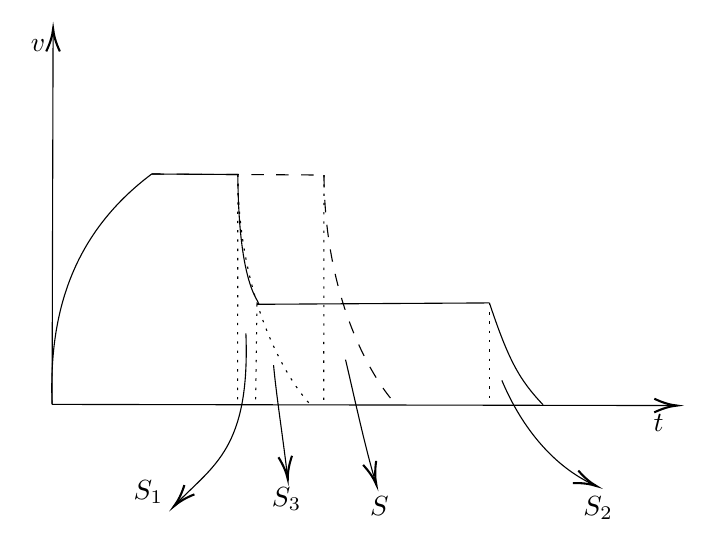
\begin{tikzpicture}[x=0.75pt,y=0.75pt,yscale=-1,xscale=1]
%uncomment if require: \path (0,300); %set diagram left start at 0, and has height of 300

%Straight Lines [id:da0857601338659093] 
\draw    (99.99,210.06) -- (100.48,31.06) ;
\draw [shift={(100.49,29.06)}, rotate = 90.16] [color={rgb, 255:red, 0; green, 0; blue, 0 }  ][line width=0.75]    (10.93,-3.29) .. controls (6.95,-1.4) and (3.31,-0.3) .. (0,0) .. controls (3.31,0.3) and (6.95,1.4) .. (10.93,3.29)   ;
%Straight Lines [id:da45900269236989355] 
\draw    (99.99,210.06) -- (399.06,210.62) ;
\draw [shift={(401.06,210.63)}, rotate = 180.11] [color={rgb, 255:red, 0; green, 0; blue, 0 }  ][line width=0.75]    (10.93,-3.29) .. controls (6.95,-1.4) and (3.31,-0.3) .. (0,0) .. controls (3.31,0.3) and (6.95,1.4) .. (10.93,3.29)   ;
%Curve Lines [id:da6769226143475053] 
\draw    (99.99,210.06) .. controls (98.49,169.06) and (107.99,129.06) .. (147.99,99.06) ;
%Straight Lines [id:da8144378967631352] 
\draw  [dash pattern={on 4.5pt off 4.5pt}]  (147.99,99.06) -- (230.99,99.56) ;
%Curve Lines [id:da4014399676965663] 
\draw  [dash pattern={on 4.5pt off 4.5pt}]  (230.99,99.56) .. controls (231.37,160.5) and (254.7,198.5) .. (266.04,210.5) ;
%Curve Lines [id:da9960457114551022] 
\draw  [dash pattern={on 0.84pt off 2.51pt}]  (189.49,99.31) .. controls (189.87,160.25) and (213.2,198.25) .. (224.54,210.25) ;
%Curve Lines [id:da2798877717119481] 
\draw    (189.49,99.31) .. controls (189.87,160.25) and (202.7,161.17) .. (198.7,161.84) ;
%Straight Lines [id:da8676574264203525] 
\draw    (198.7,161.84) -- (310.7,161.17) ;
%Curve Lines [id:da4646817563457404] 
\draw    (310.7,161.17) .. controls (320.04,189.17) and (325.2,198.25) .. (336.54,210.25) ;
%Straight Lines [id:da10287821494402793] 
\draw    (147.99,99.06) -- (189.49,99.31) ;
%Straight Lines [id:da16535020021066482] 
\draw  [dash pattern={on 0.84pt off 2.51pt}]  (189.49,99.31) -- (189.37,209.84) ;
%Straight Lines [id:da6921188479999794] 
\draw  [dash pattern={on 0.84pt off 2.51pt}]  (230.99,99.56) -- (230.87,210.09) ;
%Straight Lines [id:da4808931550760813] 
\draw  [dash pattern={on 0.84pt off 2.51pt}]  (310.7,161.17) -- (310.7,209.84) ;
%Straight Lines [id:da9648517129778311] 
\draw  [dash pattern={on 0.84pt off 2.51pt}]  (198.7,161.84) -- (198.04,210.5) ;
%Curve Lines [id:da03245337015312333] 
\draw    (193.37,175.84) .. controls (195.48,231.29) and (177.63,239.45) .. (160.05,257.74) ;
\draw [shift={(158.7,259.17)}, rotate = 312.95] [color={rgb, 255:red, 0; green, 0; blue, 0 }  ][line width=0.75]    (10.93,-3.29) .. controls (6.95,-1.4) and (3.31,-0.3) .. (0,0) .. controls (3.31,0.3) and (6.95,1.4) .. (10.93,3.29)   ;
%Curve Lines [id:da1482904002948846] 
\draw    (316.7,198.5) .. controls (324.67,217.56) and (338.81,238.31) .. (360.52,248.61) ;
\draw [shift={(362.21,249.38)}, rotate = 203.81] [color={rgb, 255:red, 0; green, 0; blue, 0 }  ][line width=0.75]    (10.93,-3.29) .. controls (6.95,-1.4) and (3.31,-0.3) .. (0,0) .. controls (3.31,0.3) and (6.95,1.4) .. (10.93,3.29)   ;
%Curve Lines [id:da3852454279932427] 
\draw    (241.37,188.5) .. controls (245.39,205.43) and (250.5,229.61) .. (255.65,246.86) ;
\draw [shift={(256.21,248.71)}, rotate = 252.9] [color={rgb, 255:red, 0; green, 0; blue, 0 }  ][line width=0.75]    (10.93,-3.29) .. controls (6.95,-1.4) and (3.31,-0.3) .. (0,0) .. controls (3.31,0.3) and (6.95,1.4) .. (10.93,3.29)   ;
%Curve Lines [id:da6433697978280477] 
\draw    (206.7,191.17) .. controls (208.15,206.81) and (211.31,226.6) .. (213.32,244.14) ;
\draw [shift={(213.54,246.04)}, rotate = 263.66] [color={rgb, 255:red, 0; green, 0; blue, 0 }  ][line width=0.75]    (10.93,-3.29) .. controls (6.95,-1.4) and (3.31,-0.3) .. (0,0) .. controls (3.31,0.3) and (6.95,1.4) .. (10.93,3.29)   ;

% Text Node
\draw (88.5,33) node [anchor=north west][inner sep=0.75pt]   [align=left] {$\displaystyle v$};
% Text Node
\draw (388.5,213.5) node [anchor=north west][inner sep=0.75pt]   [align=left] {$\displaystyle t$};
% Text Node
\draw (138,245.33) node [anchor=north west][inner sep=0.75pt]   [align=left] {$\displaystyle S_{1}$};
% Text Node
\draw (354.67,253) node [anchor=north west][inner sep=0.75pt]   [align=left] {$\displaystyle S_{2}$};
% Text Node
\draw (252,253) node [anchor=north west][inner sep=0.75pt]   [align=left] {$\displaystyle S$};
% Text Node
\draw (204.67,249) node [anchor=north west][inner sep=0.75pt]   [align=left] {$\displaystyle S_{3}$};


\end{tikzpicture}
\caption{提前进入减速阶段示意图}
\end{figure}
\begin{eqnarray}
S_1+S_2=S_1+S_3=S
\end{eqnarray}

接下来我们只需考虑改变后的匀速阶段行驶距离,假设改变后匀速阶段速度为$v'_m$,原计划匀速阶段还需运行时间$t'$,则有:
\begin{eqnarray}
v_m\cdot t'=v'_m\cdot(t'+\Delta t)
\end{eqnarray}
\begin{eqnarray}
S=s_m+(t_m+t_{m1}-t')v_m
\end{eqnarray}
其中,$\Delta t=60s$,$S=2000m$,我们就可以数值求解得到改变后的运行速度$v'$,这样我们就确定了列车的调整方案。

我们将优化调整后的曲线组展示在下图中:
\begin{figure}[H]
\centering
\includegraphics[width=.24\textwidth,height=0.24\textwidth]{figures/aaa.eps}
\includegraphics[width=.24\textwidth,height=0.24\textwidth]{figures/bbb.eps}
\includegraphics[width=.24\textwidth,height=0.24\textwidth]{figures/ccc.eps}
\includegraphics[width=.24\textwidth,height=0.24\textwidth]{figures/ddd.eps}
\caption{\song\wuhao 优化调整后的曲线组}
\end{figure}

\clearpage
\section{模型评价}
\subsection{模型优点}
\begin{enumerate}
  \item 简化列车运行几个阶段使得模型得到简化
\item 利用栅格化蚁群算法可以有效降低求解问题的复杂度 
\end{enumerate}
\subsection{模型缺点}
\begin{enumerate}
\item 龙格库塔法求数值解可能存在精度的问题使得结果精确度不能得到保证
\item 未考虑到电机的复杂动态过程可能会使模型结果产生较大偏差
\end{enumerate}

% 1. 优点

% \textcolor{red}{得到满意的解、
% 较好地解决了$\cdots$问题、
% 使模型得到简化、
% 使结果更合理,避免…带来的较大误差、
% 使问题描述比较清晰、
% 减少大的计算量。
% }

% (1)问题求解中 辅之流程图, 将建模思路完整清晰的展现出来;

% (2)问题二在对 问题二在对理论通行能力进修复时考虑因素 细致、全面,理论通行能力进修复时考虑因素
%  细致、全面,系数准确度高;

% (3)在问题三中,提出“影响度”的概念较为直观地定量给小区开放后的效果,简便有.在影响度计算上由
% 点及面从每个路段、交叉口到整 个路网,层深入具有逻辑性;

% \begin{figure}[h!t]
% \centerline{\includegraphics[scale=1]{fig4.pdf}}
% \caption{\song\wuhao 图~3的标题名称}
% \end{figure}


% (4)运用多种数学软件(如 MATLAB、SPSS),取长补短,使计算结果更加),取长补短,使计算结果更
% 加 准确、明晰.

% 2. 缺点

% \textcolor{red}{主观性过强、
% 建立在什么的前提条件下、
% 有一定的局限性、
% 存在不确定性、
% 有一定的偏差。
% }

% (1)在数学软件的计算中会将小数计算 结果进行保留,使得随后的会将小数计算 结果进行保留,使得随后
% 的或统计结果造成一定误差;

% (2)问题二求解修正通行能力时多次使用了查表,操作不够简便.

% \subsection{模型的、模型的 推广}

% \begin{itemize}

% \item \textcolor{red}{对本文中的模型给出比较客观的评价,必须实事求是,有根据,以便评卷人参考。}

% \item \textcolor{red}{推广和优化,需要花费功夫想出合理的、甚至可以合理改变题目给出的条件的、不一定可行但是具有一定想象空间的准理想的方法、模型。由此做出一些改进方向,也可以是参赛者一些来不及实现的思路。}
% \end{itemize}

% 1. 问题二中 建立 的模型 在现实 生活 中可以 作为 检验 数据 对实测数据 的准确 性进行 检验,帮助 人们
% 更好 的测算 交通 数据.

% 2. 基于问题三建立的模型,可以根据道路实时检测数(某段单位间内 基于问题三建立的模型,推算新建
% 一条道路对于当前交 通状况的改善效果,帮助度等).

% \section{模型的改进}

% \subsection{模型一的改进}
% 针对问题二中的模型一,在具体求解大型车对车辆通行能力的修正系数时,
% 我们利用交通量的测算值对照得到相应的大型车修正系数.但是,在实际操作中
% 交通量的测定有很大的难度,如果此时交通量数据无法得到,那么我们便不能得
% 到相应的修正系数,因此我们对模型进行改进.

% 由~GREENSHIELD K-V 线性模型,可得通行能力的公式:
% \begin{align}
% A_{p}=\begin{cases}
% \dfrac{3600}{t}\left(1-\dfrac{3.6 l}{V_{t} t}\right)\left(V_{f}>7.2 l / t\right) \\
% \dfrac{250 V_{f}}{t}\left(V_{f} \leq 7.2 l / t\right)
% \end{cases}
% \end{align}

% 对应的临界车辆速度:
% \begin{align}
% V_{p}=\begin{cases}
% \dfrac{V_{f}-3.6 l}{t} & \left(V_{f}>7.2 l / t\right) \\
% \dfrac{1}{2} V_{f} & \left(V_{f} \leq 7.2 l / t\right)
% \end{cases}
% \end{align}

% 由美国道路通行能力准则可得,美国将道路服务水平分为六级:A-F 级,而
% 我国目前针对当前国情,将道路服务水平分成四级:一级相当于美国的A、B 两
% 级;二级相当于美国的C 级;三级相当于美国的D 级;四级相当于美国的E、F
% 级。因此,相应的,将美国服务水平划分标准进行针对性修正,得到中国道路服
% 务水平划分标准,见表

% \begin{table*}[h!]
%   \centering
%   \small
%   \tabcolsep 2pt
%   \caption{我国服务水平划分标准}
% \begin{tabular*}{0.87\linewidth}{p{60pt}<{\centering}p{40pt}<{\centering}
% p{40pt}<{\centering}p{40pt}<{\centering}p{40pt}<{\centering}
% p{80pt}<{\centering}p{40pt}<{\centering}}
% \toprule
% 服务水平 (L0S)  & \multicolumn{2}{c} {一级 } & 二级  & 三级  & \multicolumn{2}{c} {四级 } \\
% \cline{2-3}\cline{6-7}
% 服务交通量  & 800 & 1200 & 1800 & 2500 & $A_{D}$ & $\leqslant A_{P}$ \\
%  速度  km / h & 120 & 120 & 120 & 120 & $\geqslant V_{p}$ & $\leqslant V_{p}$ \\
%  V / C & 0.33 & 0.48 & 0.71 & 1.0 & $A_{p} / A_{\max}\leqslant 1.0$ & -(无意义 ) \\
% \bottomrule
%   \end{tabular*}
% \end{table*}

% 由于车流量的测算相对于交通量来说较易得到,我们便可以不用对交通量进
% 行测算,可以通过车流量与通行能力的比值计算出~V/C 饱和度值,再通过该值对
% 照我国服务水平划分标准,间接得到服务交通量,从而得到大型车对通行能力的
% 修正系数.


% \subsection{模型二的改进}

% 针对于问题三中的模型,在得出各个类型小区在开放后对于整个小区周边路
% 网交通负荷影响度后,无法判别小区开放的效果是积极的还是消极的,由此我们
% 可以采用~Bress 悖论的原理进行判别:在个人独立选择路径的情况下,为某路网
% 增加额外的通行能力(如增加路段的等),反而会导致整个路网的整体运行水平
% 降低的情况.

% 将路网进行简化如图~15:

% 根据推导可得: 当 $\beta_{3}/\left(\beta_{1}+\beta_{2}\right) \leq\left(\beta_{5}+\beta_{6}\right)/\beta_{4}$ 时,会发生悖论,即道路的开
% 通反而会加剧原有道路的交通状况.

% \textcolor{red}{需重新起页,不得与论文正文内容在同一页上}

% \begin{rmk}
% 5篇以上!
% \end{rmk}



\begin{thebibliography}{99}
\addcontentsline{toc}{section}{参考文献}
\bibitem{__2011}
熊 康.
\newblock 高速动车组列车牵引仿真计算技术研究.
\newblock {\it 中国工程科学}, 13(1):62--68, 2011.
\newblock 45 citations(CNKI)[2023-5-14].

\bibitem{__2023}
 李兰鹏.
\newblock
  基于蚁群算法的城市轨道交通列车节能运行优化模型仿真分析.
\newblock {\it 城市轨道交通研究}, 26(2):11--15, 2023.
\newblock {\textless}北大核心{\textgreater}.

\bibitem{__2022}
 李和壁,  梁家健,  张守帅,  白鑫, and  姜昕良.
\newblock 高速铁路动车组集群运行仿真技术研究.
\newblock {\it 铁道运输与经济}, 44(10):135--143, 2022.
\newblock {\textless}北大核心{\textgreater}.

\bibitem{__2020}
李瑶 .
\newblock {\it
  基于人工蜂群算法的城轨列车运行节能优化研究}.
\newblock 硕士, 兰州交通大学, 2020.
\newblock 6 citations(CNKI)[2023-5-14].
\end{thebibliography}


% \begin{appendices}

% \section*{}

% % \textbf{\textcolor[rgb]{0.98,0.00,0.00}{程序一:MATLAB算道路车辆通行能力:}}
% % \lstinputlisting[language=Matlab]{./code/mcmthesis-matlab1.m}

% % \section*{}

% % \textcolor[rgb]{0.98,0.00,0.00}{\textbf{程序二:C++ 求解路网正体影响度:}}
% % \lstinputlisting[language=C++]{./code/mcmthesis-sudoku.cpp}

% % \newpage
% % \def\thesection{A}
% % \renewcommand{\thetable}{\wuhao A-\arabic{table}}
% % \setcounter{table}{0}
% % \section*{数据表格}
% % \textcolor[rgb]{0.98,0.00,0.00}{\textbf{表格数据:}}
% % \input{Appendices1}

% \end{appendices}
\end{document}
%%
%% This work consists of these files mcmthesis.dtx,
%%                                   figures/ and
%%                                   code/,
%% and the derived files             mcmthesis.cls,
%%                                   mcmthesis-demo.tex,
%%                                   README,
%%                                   LICENSE,
%%                                   mcmthesis.pdf and
%%                                   mcmthesis-demo.pdf.
%%
%% End of file `mcmthesis-demo.tex'.
